
%\chapter{非常规性与多样性注入的实时交通轨迹编辑}
\chapter{交互式交通仿真与轨迹编辑框架}
\label{chapter:traedits}

%自动驾驶虽然在提高人们生活质量、加快城市智能化建设等方面有着不小的潜力,然而在技术尚未成熟的今天,如何安全地落地和推广自动驾驶仍然面临着巨大的挑战。近些年来,除了在实际道路上测试和验证自动驾驶算法的性能外,一个高保真的交通仿真器能以更快捷、方便的方式提供可靠的虚拟测试环境和数据。

自动驾驶作为交通仿真的一个重要下游产业,其中一个应用便是使用仿真生成的交通场景来高效、安全地训练或测试自动驾驶算法,即自动驾驶中称呼的World-Sim。随着业界需求的不断提高,使用World-Sim来快捷、大量地创造出包含多样驾驶行为的边缘案例用于提升测试的覆盖率,成为了排查自动驾驶风险隐患、提高算法鲁棒性的重中之重。但无论是目前市面上的第三方仿真软件如SUMO~\cite{krajzewicz2002sumo},SimMobility~\cite{adnan2016simmobility},Vissim~\cite{fellendorf1994vissim}和Carla~\cite{dosovitskiy2017carla},还是图形学领域借鉴群组动画提出的可视化交通重构、仿真方法~\cite{sewall2010virtualized, wilkie2013flow, li2017city, chao2017realistic, ren2019heter},更多的都是倾向于生成常规驾驶行为的平稳交通流数据,例如保守的加减速、跟驰前车、简单的变道或是红绿灯控制等等。究其原因,一是基于规则的仿真方法很难将非常规行为发生的个体心理、生理、社交、环境等因素准确建模的同时又保证生产过程的高效;二是基于数据驱动的仿真方法则受限于采集数据中的车辆运动模式,本就无法泛化得到没有采集或是较少发生的的驾驶行为。

为了帮助自动驾驶的World-Sim高效地生成带有非常规的、多样驾驶行为的边缘案例,本研究将目光落在了人机交互领域中的交互式编辑技术。当前的交通仿真技术的另一大弊端是缺乏高质量的用户交互体验,仿真的过程几乎都是全自动、无法人为干预的,这使得仿真的结果具有非常大的不确定性,用户想要获取一些预定义的结果就需要繁琐地调试仿真器调参或场景预设,反复试错直到结果满足预期为止。而交互式编辑技术已经在人群动画中被广泛应用,动画制作者为了解决定制化结果生成的效率问题,提出了使用基于cage的变形技术~\cite{kim2014interactive}、基于网格变形技术~\cite{zhang2020crowd}或使用手绘草图~\cite{montana2017sketching}等方法让用户交互式地编辑人群动画。倘若将用户实时交互引入交通仿真的过程,便可以巧妙地将个体非常规驾驶的决策过程交由用户控制,从而弱化影响行为发生的各种因素——这不失为一个同时提高个体行为多样性和定制化数据生成效率的一石二鸟的方案。


在引入了用户编辑之后,仿真车辆可能会由于用户的引导而做出如偏离车道等不遵守交规约束的行为,同时也会不可避免地提高交通事故的发生概率。但是,本研究不着重研究非常规行为导致的交通事故场景生成,而是希望车流在引入这些行为之后车流仍然能保证相对平稳的运行,因此仍然将“碰撞避免”视为刻画车辆运动的重要因素之一,主要原因有以下几点:
\begin{itemize}
    \item 从仿真的角度来说,现实世界中的驾驶员无论是自身在非常规驾驶,还是在面对非常规行驶的邻车时,也都是希望能保持人身财产安全的;即使在危险情况下,驾驶员也会采取应急措施来避免碰撞事故,而不是仍由事故的发生;
    
    \item 从应用领域来说,自动驾驶为了保证数据的真实性,交通事故通常有专用的Log-Sim场景进行回放测试;而World-Sim的主要用于生成大量的场景来测试自动驾驶算法的反馈,或是辅助训练算法避免发生碰撞。

    %\item 从交互体验来说,在可视化交通仿真领域,事故的模拟是集多方面技术的大成,包含了碰撞的检测、特效渲染和失控行为的进一步模拟(如ragdoll技术)等等,仅从群体行为仿真的算法设计出发并不能保证视觉结果的真实性,且引入额外的计算开销也有悖于提升用户生成结果效率的初衷;
    \item 从交互体验来说,在可视化领域中模拟交通事故,除了需要大量的计算资源解算交通参与者之间复杂的物理、行为交互,还需要引入额外的特效模拟、画面渲染、失控行为(如ragdoll技术)等以保证结果在视觉上的真实性,这些都会严重拖累用户的交互体验,有悖于本文提升用户使用效率的初衷;
    
\end{itemize}


%目前发布的第三方交通仿真软件如SUMO~\cite{krajzewicz2002sumo},SimMobility~\cite{adnan2016simmobility},Vissim~\cite{fellendorf1994vissim}和Carla~\cite{dosovitskiy2017carla}都能帮助用户生成包含常规驾驶行为的平稳交通流数据。但假如用户希望生成一些非常规的交通场景,或者对已有的交通轨迹数据进行精细化调整,用户需要凭经验和已有的结果来反复调整仿真模型参数和场景预设并重新仿真,使仿真结果逐步满足预期,这是一个十分繁琐的过程。在人群动画的创作过程中,动画制作者为了解决相似的问题引入了交互编辑技术,使用基于cage的变形技术~\cite{kim2014interactive}、基于网格变形技术~\cite{zhang2020crowd}或使用手绘草图~\cite{montana2017sketching}等方法让用户交互式地编辑人群动画。相比于人群的运动,车辆运动需要满足非完备性运动学约束,加减速运动具有更大的惯性,不能像人一样瞬时改变朝向,且还有更多额外的交通规则限制,因此很难将编辑人群动画的方法直接应用到交通仿真中。

%另一方面,为了提高结果的真实性,图形学邻域近年来提出了许多数据驱动的交通仿真方法以生成街道级别的微观车辆运动,例如利用道路上架设的传感器来采集数据重构交通流~\cite{sewall2010virtualized, wilkie2013flow, li2017city},使用纹理合成的思想为任意形状的城市道路填充车流~\cite{chao2017realistic},也能扩展到混合多智能体的仿真系统~\cite{ren2019heter}。尽管结果足够真实,用户依然无法从这些方法中获取更多样和非常规的行为结果,究其原因,一是先前的方法更倾向于模拟包含常规驾驶行为的稳定车流,二是采集数据中的车辆运动模式本就单一,无法学出更复杂的行为。而在引入了交互编辑的概念之后,仿真车辆可能会由于用户的引导而做出如完全偏离车道的非常规行为,这与上述仿真方法将车辆严格控制在车道中心线附近行驶的策略相违背,如何仿真更新车辆使其运动能满足用户任意的编辑而又不失真亦是一大挑战。

因此,如何设计个体的运动控制算法和用户的交互逻辑并将二者进行合理的结合,以保证车辆的行为既满足用户预期又不失真,是一大艰巨的挑战。本章提出了一个非常规性与多样性注入的交互式交通仿真和轨迹编辑框架,命名为TraEDITS,用于高效、直观地生成用户预期的交通轨迹结果。该方法的框架中融合了一个基于优化策略的交通仿真模块和一个全局路径规划模块,并把车辆状态从全局坐标中解耦到非欧的路径坐标中表示和更新,避免了车辆运动被严格限制在车道中心线附近。通过引入交互式编辑的概念,本方法允许用户在仿真过程中实时对车辆进行控制和编辑,除了直接修改选中车辆的某些属性外,还能通过点击关键点位为车辆生成自定义的参考路径供车辆跟随。我们的方法能生成过往方法或已有数据集中很少见到的行为,例如U型掉头、跨多车道急转弯、借道超车等。本方法的主要贡献如下:

\begin{itemize}
    \item 提出了一个实时交通轨迹编辑框架,允许用户通过直观的交互操作对运动中的个体进行控制以生成预期的结果,避免了反复调整参数和仿真的繁琐试错过程。
     
    \item 提出了一种基于优化的交通个体运动控制方法,能够同时考虑用户编辑、历史交通轨迹、环境约束和物理约束等因素以满足高效快捷的轨迹编辑与生成需求。

    \item 将车辆状态从全局坐标解耦到非欧的路径坐标表示和计算,使得车辆运动更灵活,能够展现出过往方法或已有数据集中很少见到的行为。
    
\end{itemize}


\section{方法概述}

图~\ref{fig:traedits_overview}展示了本方法TraEDITS的流程。首先,我们对输入到TraEDITS中的静态场景、数据集等进行预处理,并明确车辆状态的表示方式(章节~\ref{section:traedits_coordinate})。在交通仿真模块,在考虑速度连续性、自驱动、路径保持和碰撞避免多个因素下,车辆的运动基于真实轨迹数据和能量最小化策略来更新,(章节~\ref{section:traedits_simulate});在全局路径规划模块,在使用胶囊形去逼近道路形状将场景离散化表示成网格后(章节~\ref{section:traedits_discretize}),用户使用鼠标点击的一系列关键点将作为启发式路径搜索的输入来生成新的的参考路径(章节~\ref{section:traedits_planning})。为了保证车辆在跟随用户任意指定的参考路径时运动都不失真,我们进一步添加了运动学和路径几何的约束(章节~\ref{section:traedits_physics}),以提高车辆在过弯道时的行为表现。在结果部分,我们展示了整个框架的实现细节和基于本方法生成的非常规交通轨迹(章节~\ref{section:traedits_cases}),统计分析了本方法在仿真和路径规划中的时间性能~\ref{section:traedits_performance},并且通过用户调查的方式验证了本方法能够方便快捷地生成定制化的结果(章节~\ref{section:traedits_userstudy})。

\begin{figure}[!htb]
%\setlength{\abovecaptionskip}{-0.1cm} 
%\setlength{\belowcaptionskip}{-0.45cm}
\centering
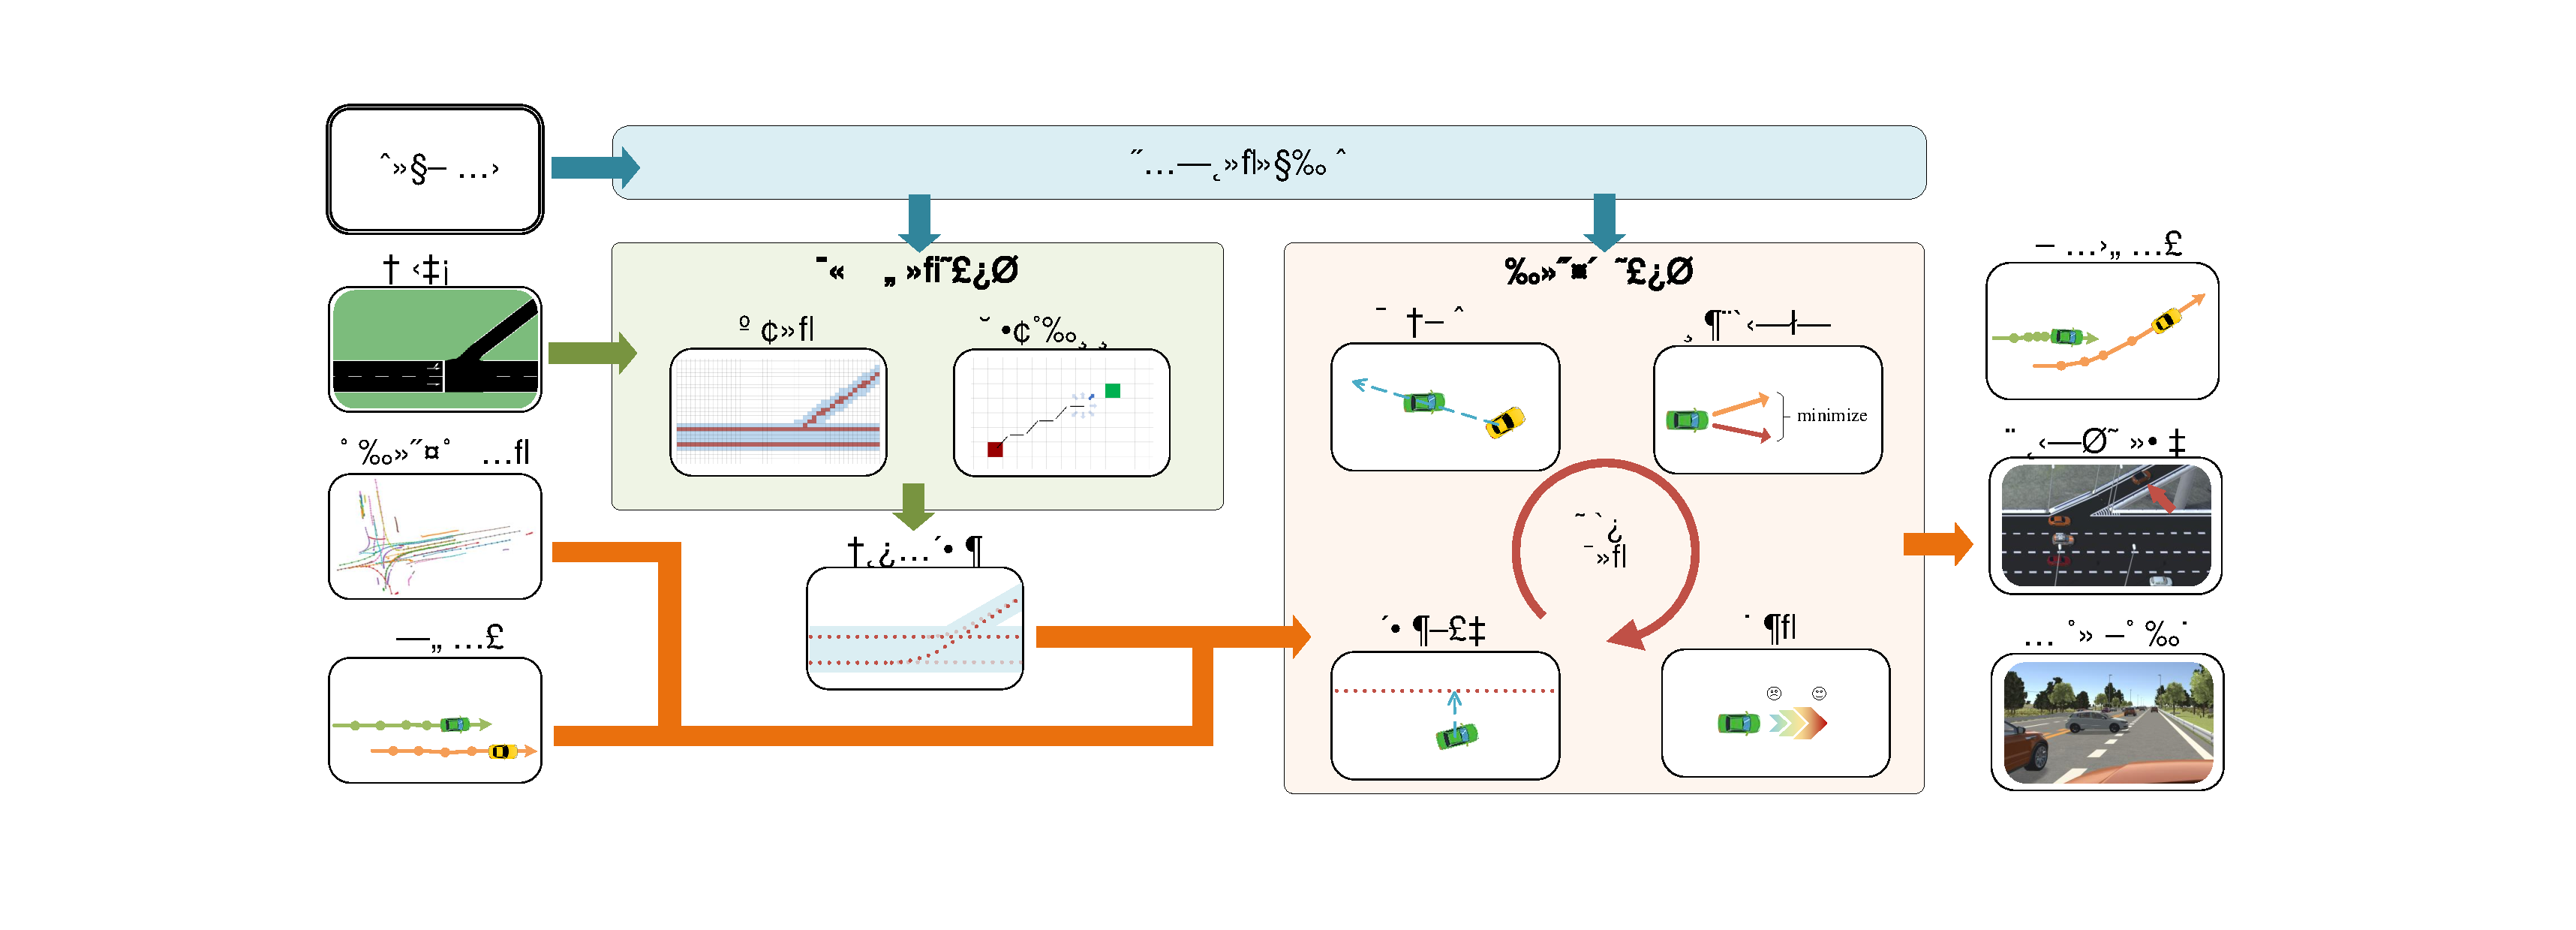
\includegraphics[width=\textwidth]{figure/traedits/overview 7_cn.pdf}
%\caption[实时交通轨迹编辑框架TraEDITS流程示意图]{
%TraEDITS框架流程示意图,包含了一个基于优化的交通仿真模块和一个全局路径规划模块。用户的编辑通过可视化图形界面收集,并传递到对应的各个模块中。}
\caption[实时交通轨迹编辑框架TraEDITS流程图]{
实时交通轨迹编辑框架TraEDITS流程图
}
\label{fig:traedits_overview}
\end{figure}


\section{坐标系与场景表示}
\label{section:traedits_coordinate}

TraEDITS同时使用Cartesian坐标系和Frenet坐标系来描述车辆的运动状态。给定一个参考路径,车辆的状态在Frenet坐标系中记为$(s, d)$,其中$s$表示沿着参考路径的纵向位移,$d$表示偏离参考线的横向距离。本方法使用$\textbf{\emph{p}}^{C}=[x, y]$, $\textbf{\emph{v}}^{C}=[v^x, v^y]$, $\textbf{\emph{p}}^{F}=[s, d]$,和 $\textbf{\emph{v}}^{F}=[v^s, v^d]$分别表示车辆在Cartesian坐标系和Frenet坐标系中的位置和速度。

此外,TraEDITS对“车道”和“路径”的定义不同。一条车道表示车辆能够行驶的一片静态区域,通常由一段一段的节点组成,在用户给定的场景文件中定义,多条车道首尾相连组成了完整的道路网络。我们记一条车道为$\mathscr{L}_i = [\textbf{Q}^{\mathscr{L}}_{i}, w_i, \textbf{T}_{i}]$,其中$\textbf{Q}^{\mathscr{L}}_{i}$表示在Cartesian坐标系中每一段节点的位置集合,$w_i$表示车道宽度,$\textbf{T}_{i}$则表示当前车道与其他车道之间的拓扑关系,包括入车道、出车道和邻车道。一条路径则用于平滑连接两个特定的位置,通常是一系列从出发点到终点的顺序点集合,可以动态地生成。我们记一条路径为$\mathscr{P}_i = [\textbf{Q}^{\mathscr{P}}_{i}, \textbf{S}_{i}, \textbf{C}_{i}]$,其中$\textbf{Q}^{\mathscr{P}}_{i}$表示组成路径的点集合,$\textbf{S}_{i}$表示对点集插值所使用的三次样条函数,$\textbf{C}_{i}$则表示路径中包含的一段段曲线部分,分别包含每一段的起点、终点、中心点和半径。值得注意的是,路径点集$\textbf{Q}^{\mathscr{P}}_{i}$的坐标可以通过三次样条函数$\textbf{S}_{i}$在Cartesian坐标系和Frenet坐标系之间相互转换。

假设在一个场景中存在$K$条车道,车道的集合表示为$\mathscr{L}^* = [\mathscr{L}_0, \mathscr{L}_1,...\mathscr{L}_K]$。我们将车道的集合$\mathscr{L}^*$所包含的车道拓扑信息转变为一张有向图,用于表征每条车道的入车道、出车道和邻车道,并将路径的集合初始化为$\mathscr{P}^* = {\mathscr{P}^*_{topo}}\cup{\mathscr{P}^*_{user}}$,$\mathscr{P}^*_{topo} = DFS\left(\mathscr{L}^*\right)$和$\mathscr{P}^*_{user} = \varnothing$分别表示由车道拓扑信息和用户自定义生成的参考路径,其中$DFS$操作表示深度优先搜索。对任意路径$\mathscr{P}_{i}\in\mathscr{P}^*_{topo}$,我们通过使用深度优先搜索来确定组成路径的点集合$\textbf{Q}^{\mathscr{P}}_{i}$,并生成对应的三次样条插值函数$\textbf{S}_{i}$。最终,每一条路径$\mathscr{P}_{i}\in\mathscr{P}^*_{topo}$都是一条从某个无入车道起点,到个某无出车道终点的唯一连接。




\section{数据驱动的交通仿真方法}
\label{section:traedits_simulate}

对没有被编辑,或者不在被编辑车辆邻域范围内的车辆,我们倾向于不改变其原先的行为,因此使用他们原先的轨迹信息更新他们的状态和运动。而对于那些被编辑,或者已经受被编辑车辆影响的车辆,我们考虑使用基于能量优化的交通仿真方法来更新他们的状态,以保证其运动符合用户的编辑输入,或者对被编辑车辆的行为变化做出正确的反馈。

本方法包含的数据驱动的基于能量优化的交通方法过程如下。首先,我们将真实采集的交通轨迹数据进行预处理得到优化候选状态集合$D=\cup_{v}d_{v}$,其中$d_v=[\textbf{\emph{v}}^{F}]$,而$\textbf{\emph{v}}^{F}$表示将数据集包含的轨迹速度转换到Frenet坐标系表示。在一个包含$N$辆车的场景中,任意车辆$i$ $(i=1,...,N)$在时刻$t$时的状态表示为$s_{i,t}=[\textbf{\emph{p}}^{F}_{i,t}, \textbf{\emph{p}}^{C}_{i,t}, \textbf{\emph{v}}^{F}_{i,t}, o_{i,t}, e_{i,t}, \mathscr{P}_{k,t}, \delta_{i,t}]$,其中$\textbf{\emph{p}}^{F}_{i,t}$,  $\textbf{\emph{p}}^{C}_{i,t}\in\mathbb{R}^2$分别表示车辆$i$当前时刻在Cartesian坐标系和Frenet坐标系中的位置,$\textbf{\emph{v}}^{F}_{i,t}\in\mathbb{R}^2$表示车辆$i$当前时刻在Frenet坐标系中的速度,$o_{i,t}\in\mathbb{R}$为欧拉角表示的车辆$i$当前时刻的朝向,$e_{i,t}\in\mathbb{R}$表示在无前车阻挡的情况下车辆$i$期望在道路上行驶的最大速度大小,$\mathscr{P}_{k,t}\in\mathscr{P}^*$表示车辆$i$当前跟随行驶的参考路径,$\delta_{i,t}\in\mathbb{R}$表示车辆$i$当前期望与参考路径中心保持的横向偏移距离。车辆$i$的状态更新表示为:
\begin{equation}
\setlength\abovedisplayskip{6pt}
\setlength\belowdisplayskip{6pt}
\begin{aligned}
    &\textbf{\emph{v}}^{F}_{i,t+1} = \mathop{\arg\min}\limits_{\textbf{\emph{v}}^{F}\in{d}_{v}\in{D}} \mathcal{E}(s_{i,t}), \\
    &\textbf{\emph{p}}^{F}_{i,t+1} = \textbf{\emph{p}}^{F}_{i,t} + \textbf{\emph{v}}^{F}_{i,t+1} \cdot \Delta{t}, \\
    &[\textbf{\emph{p}}^{C}_{i,t+1}, o_{i,t+1}] = \textbf{S}_{k}(\textbf{\emph{p}}^{F}_{i,t+1}), \\ %, \quad \textbf{S}_{k}\in\mathscr{P}_k \\
    &[e_{i,t+1}, \mathscr{P}_{k,t+1}, \delta_{i,t+1}] = \mathcal{G}_{i,t+1},
\end{aligned}
\label{eq:traedits_dynamics}
\end{equation}
其中$\textbf{\emph{v}}^{F}\in{d}_{v}\in{D}$为从候选集合$D$中选取的能够最小化能量函数$\mathcal{E}$的最优候选速度,并在Frenet坐标系中将车辆$i$下一$t+1$时刻的速度$\textbf{\emph{v}}^{F}_{i,t+1}$更新为$\textbf{\emph{v}}^{F}$,同时更新下一时刻车辆的位置$\textbf{\emph{p}}^{F}_{i,t+1}$。在得到Frenet坐标系中的速度和位置后,我们通过车辆$i$当前跟随的参考路径$k$的样条曲线函数$\textbf{S}_{k}$来更新车辆在Cartesian坐标下的速度,位置和朝向信息。符号$\mathcal{G}_{i,t+1}$表示一个集合,包含用户可实时编辑的部分变量值,以及由参考路径曲线计算得到的运动学约束和几何约束。能量函数$\mathcal{E}$定义为:
\begin{equation}
\setlength\abovedisplayskip{6pt}
\setlength\belowdisplayskip{6pt}
    \mathcal{E} = \emph{w}_{d} \mathcal{E}_{d} + \emph{w}_{c} \mathcal{E}_{c} + \emph{w}_{k} \mathcal{E}_{k} + \emph{w}_{a} \mathcal{E}_{a},
\label{eq:traedits_energyfunc}
\end{equation}
其中$\mathcal{E}_{d}$表示驱动车辆以预期速度行驶的自驱动项,$\mathcal{E}_{c}$表示平滑车辆速度变化的速度连续项,$\mathcal{E}_{k}$表示让车辆保持跟随当前参考路径的路径保持项,$\mathcal{E}_{a}$表示让车辆与邻车避免发生碰撞的碰撞避免项。$\emph{w}_{d}, \emph{w}_{c}, \emph{w}_{k}, \emph{w}_{a}$分别是上述每一项的权重系数。

\textbf{自驱动项:}如前文所述,在无前车阻挡的情况下,每一辆车都有一个期望在道路上行驶的最大速度,也称之为预期速度。自驱动项的目标即保证车辆按照这一预期速度在道路上行驶,其定义为:
\begin{equation}
\setlength\abovedisplayskip{6pt}
\setlength\belowdisplayskip{6pt}
    \mathcal{E}_{d} = e^{\left| ||\emph{\textbf{v}}^{F}|| - e_{i,t} \right| },
\label{eq:traedits_internaldrive}
\end{equation}
其中${e}_{i,t}$即车辆$i$在时刻$t$下的预期速度大小,该值可通过用户编辑进行实时更改,如表达式~\ref{eq:traedits_dynamics}所示。

\textbf{速度连续项:}受运动模型限制,车辆无法在一个很短的时间内突然发生很大的速度变化,速度连续项的目标即保证车辆状态更新前后的速度差异尽可能小,其定义为:
\begin{equation}
\setlength\abovedisplayskip{6pt}
\setlength\belowdisplayskip{6pt}
    \mathcal{E}_{c} = e^{ \left| ||\emph{\textbf{v}}^{F}|| - ||\emph{\textbf{v}}^F_{i,t}|| \right| } + e^{||\emph{\textbf{v}}^{F} - \emph{\textbf{v}}^F_{i,t}||},
\label{eq:traedits_velcontinuity}
\end{equation}
其中第一项为衡量速度大小的变化,第二项为衡量速度方向的变化,$\emph{\textbf{v}}^F_{i,t}$为车辆当前时刻Frenet坐标系中的速度。

\textbf{路径保持项:}在现实生活中车辆通常会沿着车道中心线行驶,但在我们的工作中我们希望车辆能够沿着参考路径行驶而非车道中心线,因为用户交互生成的自定义参考路径并不一定总是落在车道中心线附近。路径保持项即用于让车辆沿着任意参考路径行驶,其定义为:
\begin{equation}
\setlength\abovedisplayskip{6pt}
\setlength\belowdisplayskip{6pt}
    \mathcal{E}_{k} = e^{\left|  \emph{v}^{d} \Delta{t} - \delta_{i,t}  \right|},
\label{eq:traedits_pathkeeping}
\end{equation}
其中$\emph{v}^{d}\in\textbf{\emph{v}}^{F}$是Frenet候选速度的横向分量,$\delta_{i,t}$是车辆$i$在当前时刻$t$下期望与其跟随的参考路径保持的横向偏移距离,该值与车辆当前跟随的参考路径均可通过用户编辑进行实时更改,如表达式~\ref{eq:traedits_dynamics}所示。

\textbf{碰撞避免项:}车辆应当避免与过于接近的邻近车辆发生碰撞。在跟驰模型中,车辆在被堵塞而制动后不会紧挨着其他车辆,而是倾向于与其均保持一个相对安全的跟车距离,因此我们把碰撞避免作为能量优化的一部分进行求解,可以更平滑、真实地实现上述行为。碰撞避免项定义如下:
\begin{equation}
\setlength\abovedisplayskip{6pt}
\setlength\belowdisplayskip{6pt}
    \mathcal{E}_{a} = \frac{1}{||\mathscr{N}_{t}||} \sum\nolimits_{j\in\mathscr{N}_{t}} \emph{w}_{i,j} \cdot e^{ l - || \Hat{ \emph{\textbf{p}}}^{C}_{j,t+1} - \Hat{\emph{\textbf{p}}}^{C}_{i,t+1} || },
\label{eq:traedits_collisionavoid}
\end{equation}
其中$j$是在时刻$t$时属于车辆$i$的邻近车辆集合$\mathscr{N}_{t}$的任意车辆,$l$是一个截断距离,用于计算邻近车辆的相互作用时定义一个影响的最大距离上限,$\emph{w}_{i,j}$是车辆$i$和$j$之间相互影响的权重,设置为$i$的运动方向与从$i$指向$j$方向夹角的余弦,当该余弦值计算结果为负时将强制其等于0。$\Hat{ \emph{\textbf{p}}}^{C}_{i,t+1}$和$\Hat{ \emph{\textbf{p}}}^{C}_{j,t+1}$分别是车辆$i$和$j$下一时刻$t+1$时在Cartesian坐标系中的预期位置,$\Hat{ \emph{\textbf{p}}}^{C}_{i,t+1}$由假设车辆$i$以速度$\textbf{\emph{v}}^{F}$行驶得到,而$\Hat{ \emph{\textbf{p}}}^{C}_{j,t+1}$由假设车辆$j$保持其当前速度行驶得到。

与Ren等人的工作~\cite{ren2019heter}相比,我们使用Cartesian坐标系和Frenet坐标系混合的方式表示和更新车辆的状态,将车辆运动从严格沿着车道中心线行驶的限制中解耦出来,从而实现更多样化的车辆行为和交互。同时,我们将可调参数如预期速度、横向偏移距离和参考路径融入到了能量函数中,为用户的实时交互控制和编辑提供了基本的接口,建立了车辆属性编辑与行为变化之间的直观联系。





\section{交互式参考路径规划}

TraEDITS中的全局路径规划模块提供了另一种交互方式,让用户能够动态地生成自定义的参考路径供车辆跟随。对于一个给定的静态场景,整个场景空间首先会被离散化成二维的网格表示,每个网格单元中存储了车道和车辆的实时信息。然后用户能够通过鼠标点击一系列有序的关键点,这些关键点会映射到网格中,用于启发式路径搜索算法中搜索新的路径。

\subsection{场景离散化}
\label{section:traedits_discretize}

整个场景被视为一个二维平面并进行如下离散化过程:
\begin{enumerate}
    \item 计算包含场景中所有车道的包围盒以确定离散化范围,基于给定的分辨率将平均分割为若干网格单元,所有网格单元均被初始化标记为不可行驶区域。

    \item 对于每一条车道$\mathscr{L}_i = [\textbf{Q}^{\mathscr{L}}_{i}, w_i, \textbf{T}_{i}]$,取集合$\textbf{Q}^{\mathscr{L}}_{i}$中的每一对相邻的节点对,在两个节点位置分别以车道宽度$w_i$为半径生成圆形,使用分别与两个圆形相切的线段连接两个圆形,这样的线段共有两条,最终生成一个胶囊形状的区域,将胶囊状所覆盖的区域标记为可行驶区域。

    \item 将包含粗糙可行驶区域的网格整体视为二值图,使用膨胀和腐蚀的数字图像处理操作对图像进行过滤,以修复因欠采样和几何近似而形成的孔洞。

    \item 对于每一条车道$\mathscr{L}_i$所包含的节点集合$\textbf{Q}^{\mathscr{L}}_{i}$使用三次样条进行平滑插值并等距离采样,在包含完善的可行驶区域的网格中将采样得到的点进一步标记为车道中心线。
\end{enumerate}

经过上述离散化过程后,整个场景和车道信息被编码到一个二维网格中,包含了不可行驶区域、可行驶区域和车道中心区域,如图~\ref{fig:traedits_laneapproximate}所示,这些信息将用于后续参考路径的生成。此外,网格单元还将用于存储交通仿真模块中车辆的实时信息,以提高车辆邻域个体搜索的效率。

\begin{figure}[!tbh]
\centering
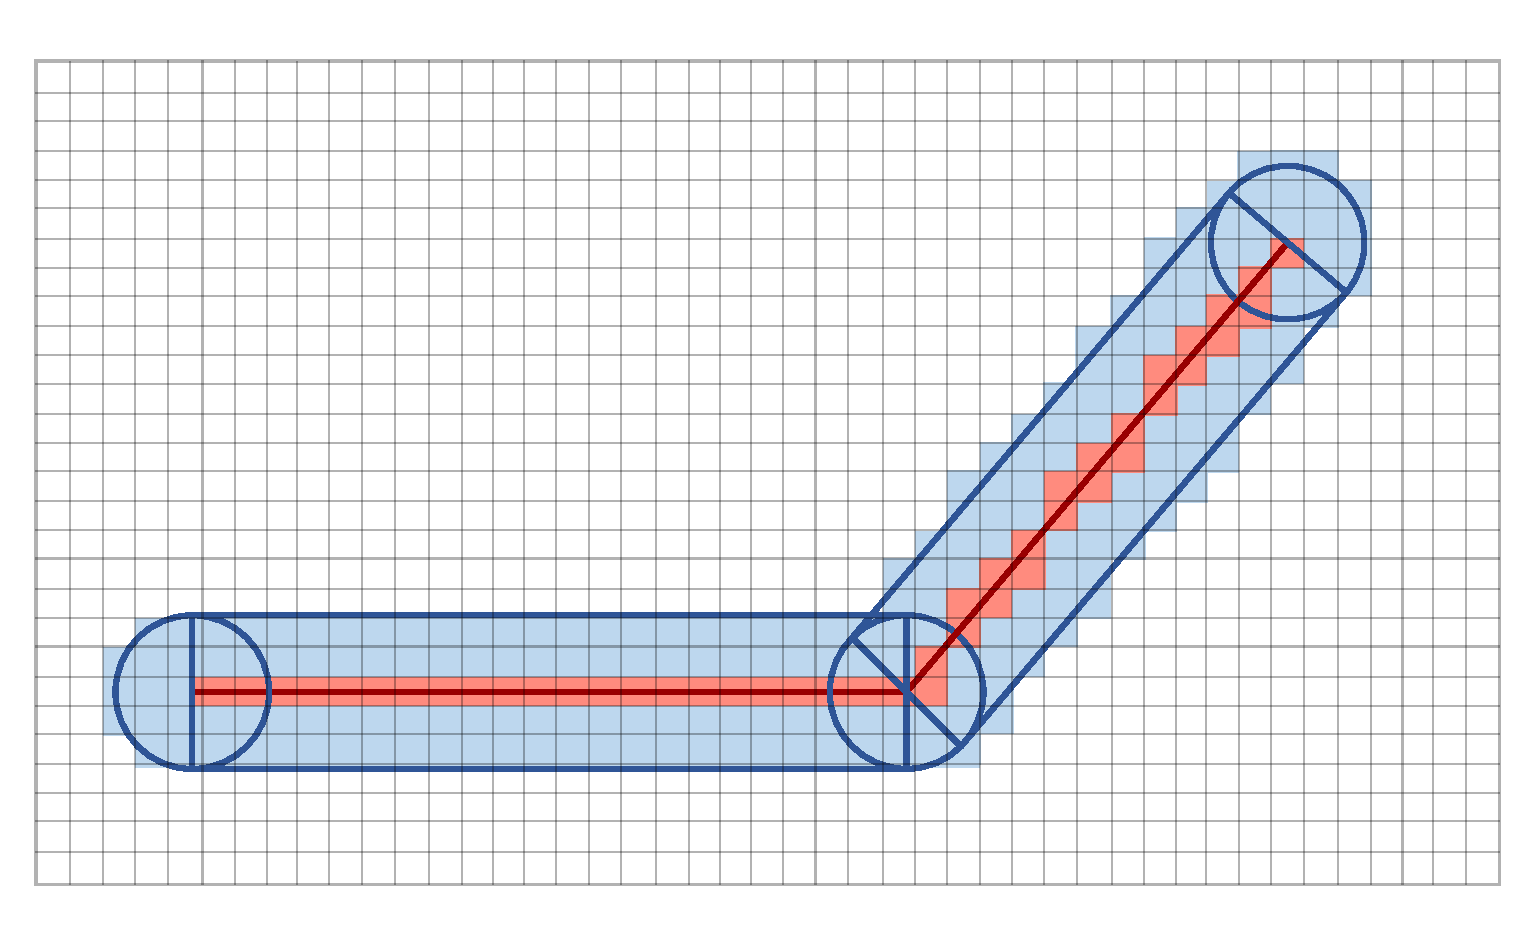
\includegraphics[width=0.9\columnwidth]{figure/traedits/lane approximation.pdf}
%\caption[基于胶囊形状的车道离散化示意图]{对于一条车道中的每一段节点对,基于胶囊形状离散化表示车道的几何形状,其中白色的区域表示不可行驶区域,蓝色的区域表示可行驶的区域,红色的区域表示车道中心线区域。}
\caption[基于胶囊状的车道离散化与几何近似]{
基于胶囊状的车道离散化与几何近似
}
\label{fig:traedits_laneapproximate}
\end{figure}




\subsection{参考路径生成}
\label{section:traedits_planning}

在离散化得到包含场景信息的网格之后,用户可以通过鼠标点击一系列有序的关键点位,基于启发式路径搜索生成自定义的参考路径$\mathscr{P}_i = [\textbf{Q}^{\mathscr{P}}_{i}, \textbf{S}_{i}, \textbf{C}_{i}]$。具体来说,首先我们将这些关键点依次映射到网格的对应单元中。其次,我们为每两个关键点之间分别生成单独的一段路径,其中第一个关键点为路径的起点,第二个关键点为路径的终点。我们使用A*路径规划算法来搜索从起点到终点的路径,并将其启发式函数修改为:
\begin{equation}
\setlength\abovedisplayskip{6pt}
\setlength\belowdisplayskip{6pt}
    g(\textbf{n}) = || \textbf{n} - \textbf{n}_{goal} || + \alpha \cdot e^{\left( \beta \cdot \rm{sign} \right)},
\label{eq:traedits_planingheuristic}
\end{equation}
其中第一项$|| \textbf{n} - \textbf{n}_{goal} ||$是当前网格单元到终点对应网格单元的欧式距离,第二项是保证路径规划的过程倾向于沿着道路中心线。$\rm{sign} \in [0,1,2]$是前述离散化过程中每个网格单元最终标签的对应数值,0代表不可行驶区域,1代表可行驶区域,2代表车道中心线区域。$\alpha$, $\beta$是两个可调的参数用于调整控制路径规划的结果。 

我们进一步对规划后的粗糙路径进行降采样,并对降采样后得到的点集合$\textbf{Q}^{\mathscr{P}}_{i}$进行高斯滤波和三次样条函数$\textbf{S}_{i}$插值,从而使得最终的参考路径足够平滑。最终,该自定义的参考路径可供用户实时指派给选定车辆跟随,即$\mathscr{P}^*_{user}=\mathscr{P}^*_{user} \cup [\mathscr{P}_{i}]$。




\section{约束计算}

由于我们使用了Cartesian坐标系和Frenet坐标系混合表示状态的方式更新车辆运动,车辆的运动从静态车道的限制中解耦出来,使其能够沿着任意的参考路径行驶。但是这样处理存在一定问题,即在现实生活中车辆在跟随不同形状的路径时通常会采取不同的运动,例如在经过一个非常急的弯道时会减速或刹车以保证安全和舒适性。为此,我们进一步计算了额外来自车辆运动学和路径几何的约束以优化车辆在跟随不同形状参考路径时的运动表现质量。

\subsection{参考路径中的曲线段鉴别}

如图~\ref{fig:traedits_curveillustration}(a)所示,鉴别一条路径$\mathscr{P}_i$中的曲线段,即根据路径的节点$\textbf{Q}^{\mathscr{P}}_{i}$和其三次样条插值函数$\textbf{S}_{i}$,找到该路径中每一段曲线段的起点、终点、中心和半径$R$,以建立路径参数中包含的$\textbf{C}_{i}$。具体的过程如下:

\begin{enumerate}
    \item 对整条路径进行等距离采样,并为每个采样点计算其曲率值。

    \item 遍历上述每个采样点,当采样点的曲率值从0变为非0值时,将该点标记为起点,然后寻找对应的曲率值从非0值变为0的采样点,将该点标记为终点与起点配对,二者之间的路径即为一个完整的曲线段。

    \item 根据该曲线段的起点和终点坐标,为其计算中心的坐标和半径$R$~\cite{li2012automated}。
\end{enumerate}

值得注意的是,我们会在获取所有的曲线段后对其进行二次判断,将长度小于给定阈值的曲线段进行舍弃,以避免一些因关键点人工指定误差或降采样后处理而引起的局部曲率突变。

\begin{figure}[t]
\centering
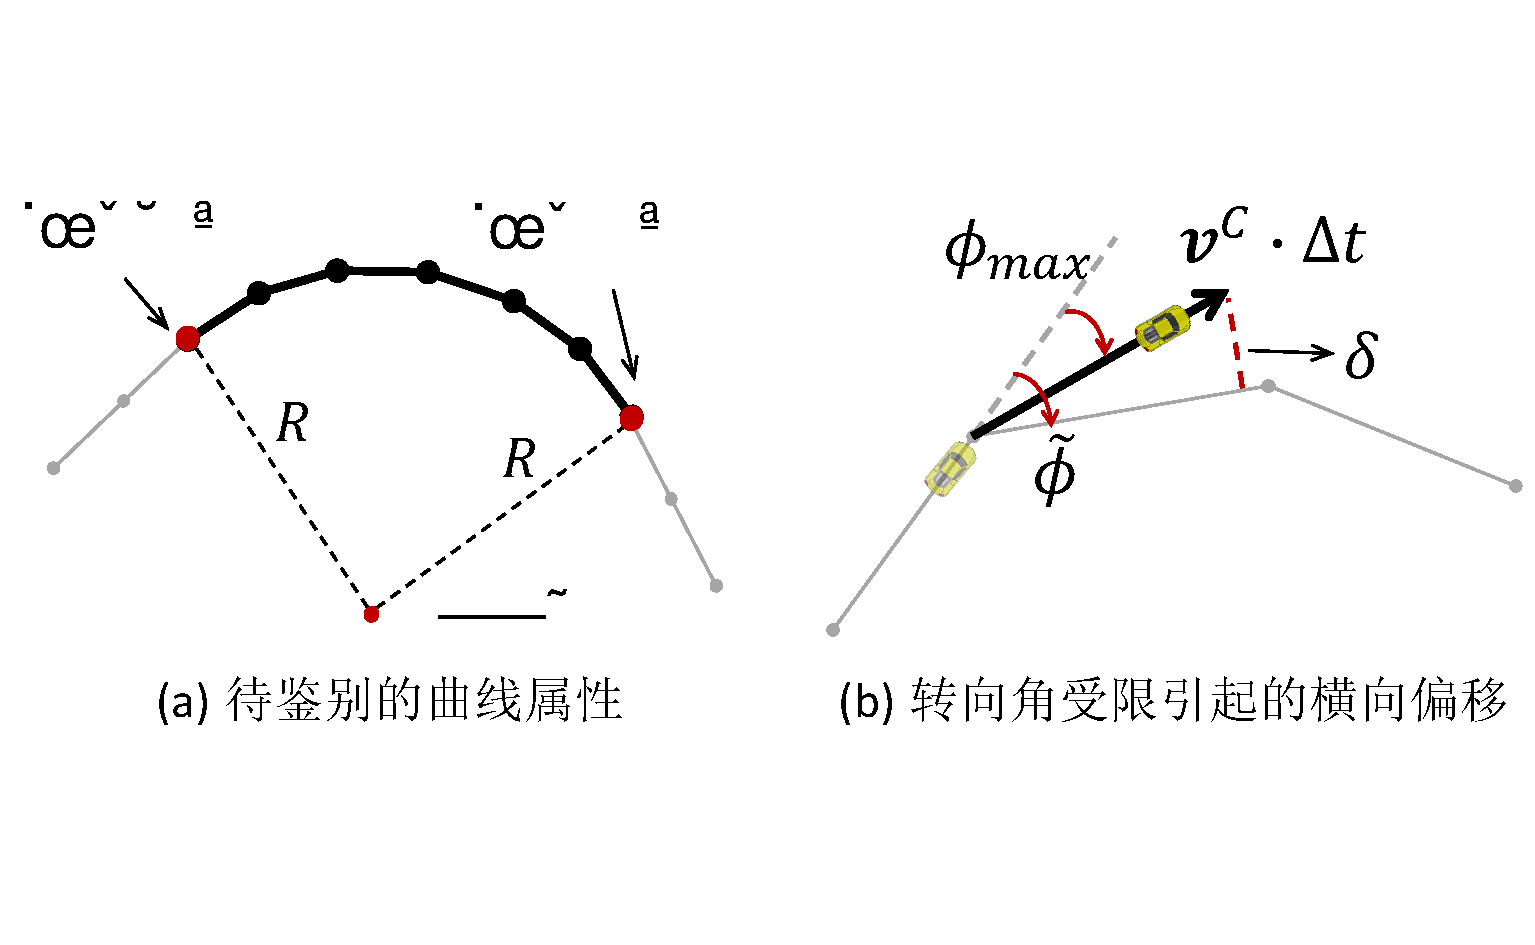
\includegraphics[width=0.7\columnwidth]{figure/traedits/curve combine 4_cn_v2.pdf}
%\caption[曲线段鉴别与转向角约束示意图]{(a) 一段经过鉴别的曲线段与其对应的起点,终点,中心和半径R。(b) 由转向角限制而引起的横向偏移$\delta$。}
\caption[曲线鉴别与车辆曲线路径跟随]{
曲线鉴别与车辆曲线路径跟随
}
\label{fig:traedits_curveillustration}
\end{figure}

\subsection{横向偏移与安全过弯速度}
\label{section:traedits_physics}

一辆车在改变方向时会受转向角的限制,因此在通过非常弯曲的路段时会因无法及时转向而发生偏移道路中心的情况。定义转向角$\phi$为车轮转动的方向与车辆朝向的夹角,而通常一辆车的转向角客观存在一个最大限制,即$|\phi| < \phi_{\rm{max}}$。我们为通过急转路径的车辆定义了一个临时的横向偏移距离:
\begin{equation}
\setlength\abovedisplayskip{6pt}
\setlength\belowdisplayskip{6pt}
    \Tilde{\delta}_{i,t} = {||\textbf{\emph{v}}^{C}_{i,t} \Delta{t}||} \cdot \sin\left( \max ( |\Tilde{\phi}| - \phi_{\rm{max}},  0 ) \right),
\label{eq:traedits_laterldeviation}
\end{equation}
其中$\Tilde{\delta}_{i,t}$表示车辆$i$在过某一曲线段时的临时横向偏移距离,$\Tilde{\phi}$表示通过该曲线段时不发生横向偏移所需要的转向角,$\phi_{\rm{max}}$表示车辆$i$所能达到的最大转向角。当$|\Tilde{\phi}| > \phi_{\rm{max}}$时,车辆会从参考路径上偏移对应的距离,而不是严格沿着路径行驶,如图~\ref{fig:traedits_curveillustration}(b)所示。

此外,驾驶员在车辆转弯时会为了安全和舒适而降低行驶速度,防止车辆因惯性而严重偏离车道发生事故。我们为路径中的每一段曲线段计算了一个安全过弯速度~\cite{gamez2017dynamic},并在有车辆驶过该段时将车辆的预期速度赋值为该安全速度,进一步提高车辆过弯行为的真实感。计算公式如下:
\begin{equation}
\setlength\abovedisplayskip{6pt}
\setlength\belowdisplayskip{6pt}
    \Tilde{e}_{i,t} = \sqrt{\left( \mu + \tan \theta  \right)g R},
\label{eq:traedits_safespeed}
\end{equation}
其中$\mu$表示车道的摩擦系数,$\theta$表示车道的倾斜角度,$g$表示重力加速度,$R$表示该段曲线段的半径。

上述两个额外的物理约束将添加到~\ref{eq:traedits_dynamics}所示的编辑集合$\mathcal{G}_{i,t} = \mathcal{G}_{i,t} \cup [\Tilde{\delta}_{i,t}, \Tilde{e}_{i,t}]$中,并比用户的实时编辑拥有更高的生效优先级以保证编辑后轨迹的质量。





\section{实验结果}

\subsection{实现细节}




实验所用设备为一台台式电脑,配置了8核的3.60GHz Intel(R) Xeon(R) W-2123处理器以及32GB的内存。TraEDITS框架的核心基于C++实现,编译成64位的动态链接库后导入到Unity3D中,进行用户图形界面的搭建与编辑仿真结果的可视化。我们在仿真模块中,使用了并行计算的方式同时更新多辆车的状态,以提高算法的运行效率。表~\ref{tab:traedits_parameters}展示了TraEDITS框架中所用到的一些重要参数的设置,这些参数初始化定义在JSON文件中并在程序运行时进行动态加载。

\begin{table}[!tbh]
\setlength{\belowcaptionskip}{.4cm}
%\setlength{\abovecaptionskip}{-0.1cm}
\centering
%\small
\renewcommand\arraystretch{1.8}
\caption[TraEDITS框架中重要参数的取值]{TraEDITS框架中重要参数的取值}
\begin{tabular}{|c|c|c|c|}
\hline
\textbf{参数} & \textbf{取值} & \textbf{单位} & \textbf{描述}                                                         \\ \hline
$\emph{w}_d$    & 1.0 & -         & 表达式~\ref{eq:traedits_energyfunc}中自驱动项的权重      \\ \hline
$\emph{w}_c$    & 0.5 & -         & 表达式~\ref{eq:traedits_energyfunc}中速度连续项的权重 \\ \hline
$\emph{w}_k$    & 10.0 & -         & 表达式~\ref{eq:traedits_energyfunc}中路径保持项的权重        \\ \hline
$\emph{w}_a$    & 5.0 & -         & 表达式~\ref{eq:traedits_energyfunc}中碰撞避免项的权重 \\ \hline
$l$                &        15.24        & $m$        & 表达式~\ref{eq:traedits_collisionavoid}中的截断距离 \\ \hline
$\alpha$           &        20.0        & \multirow{2}{*}{-}             & \multirow{2}{*}{表达式~\ref{eq:traedits_planingheuristic}中启发式搜索的权重}  \\ 
$\beta$  & -1.5 &          &                                                        \\ \hline
%$\sigma$ &  & -         &                                                        \\
$\phi_{max}$       &        30.0        & 度      &  表达式~\ref{eq:traedits_laterldeviation}中车辆的最大转向角                   \\ \hline
$\mu$    & 1.0 & -         & 表达式~\ref{eq:traedits_safespeed}中车道的摩擦系数                \\ \hline
$\theta$ & 0.0 & 度  & 表达式~\ref{eq:traedits_safespeed}中车道的倾斜角度              \\ \hline
$g$      & 9.8 & $m/s^{2}$ & 表达式~\ref{eq:traedits_safespeed}中的重力加速度 \\ \hline         
\end{tabular}
\label{tab:traedits_parameters}
\end{table}



实验所用的真实交通轨迹数据来自Next Generation Simulation (NGSIM)~\cite{alexiadis2004next},在使用这些数据之前我们对其进行了过滤以去除噪声影响。

实验所用的测试场景有两个,均使用SUMO NetEdit手动生成并导出为XML文件。第一个场景中是一个高速公路和一条离开高速公路的匝道,匝道为单车道,主路为同向的四车道。整个场景包围盒规模为977.1$\times$103.7(米),其中12.84\%为可行驶区域,1.23\%为车道中心线区域。第二个场景中是一个十字路口,每一个方向为双向四车道。整个场景包围盒规模为572.2$\times$423.6(米),其中5.16\%为可行驶区域,0.51\%为车道中心线区域。场景的离散化分辨率均为0.3$\times$0.3(米)。

图~\ref{fig:traedits_gui}中展示了我们在Unity3D中搭建的用户图形界面,用于收集用户的实时输入并传递给交通仿真模块与路径规划模块。TraEDITS运行时,用户可以使用键鼠操作移动视窗,框选一个特定的车辆$i$,其属性窗口将会显示在右上角。一些车辆属性如预期速度$e_{i}$,横向偏移距离$\delta_{i}$和当前跟随的参考路径$\mathscr{P}_{k}$可以实时修改。用户的编辑会被标注好生效的时间戳$t$然后加入到编辑集合内,即$\mathcal{G}_{i,t} = \mathcal{G}_{i,t} \cup [e_{i,t}, \mathscr{P}_{k,t}, \delta_{i,t}]$,随着仿真时间的推移对应的编辑记录会依次更新生效,如表达式~\ref{eq:traedits_dynamics}所示。在路径规划模式下,用户可以用鼠标在道路上点击关键点,用于生成自定义的参考路径,在该模式下路径平滑后处理的参数也可以进行修改。


\begin{figure}[!tbh]
%\setlength{\abovecaptionskip}{-0.05cm} 
%\setlength{\belowcaptionskip}{-0.5cm}
\centering
\centering
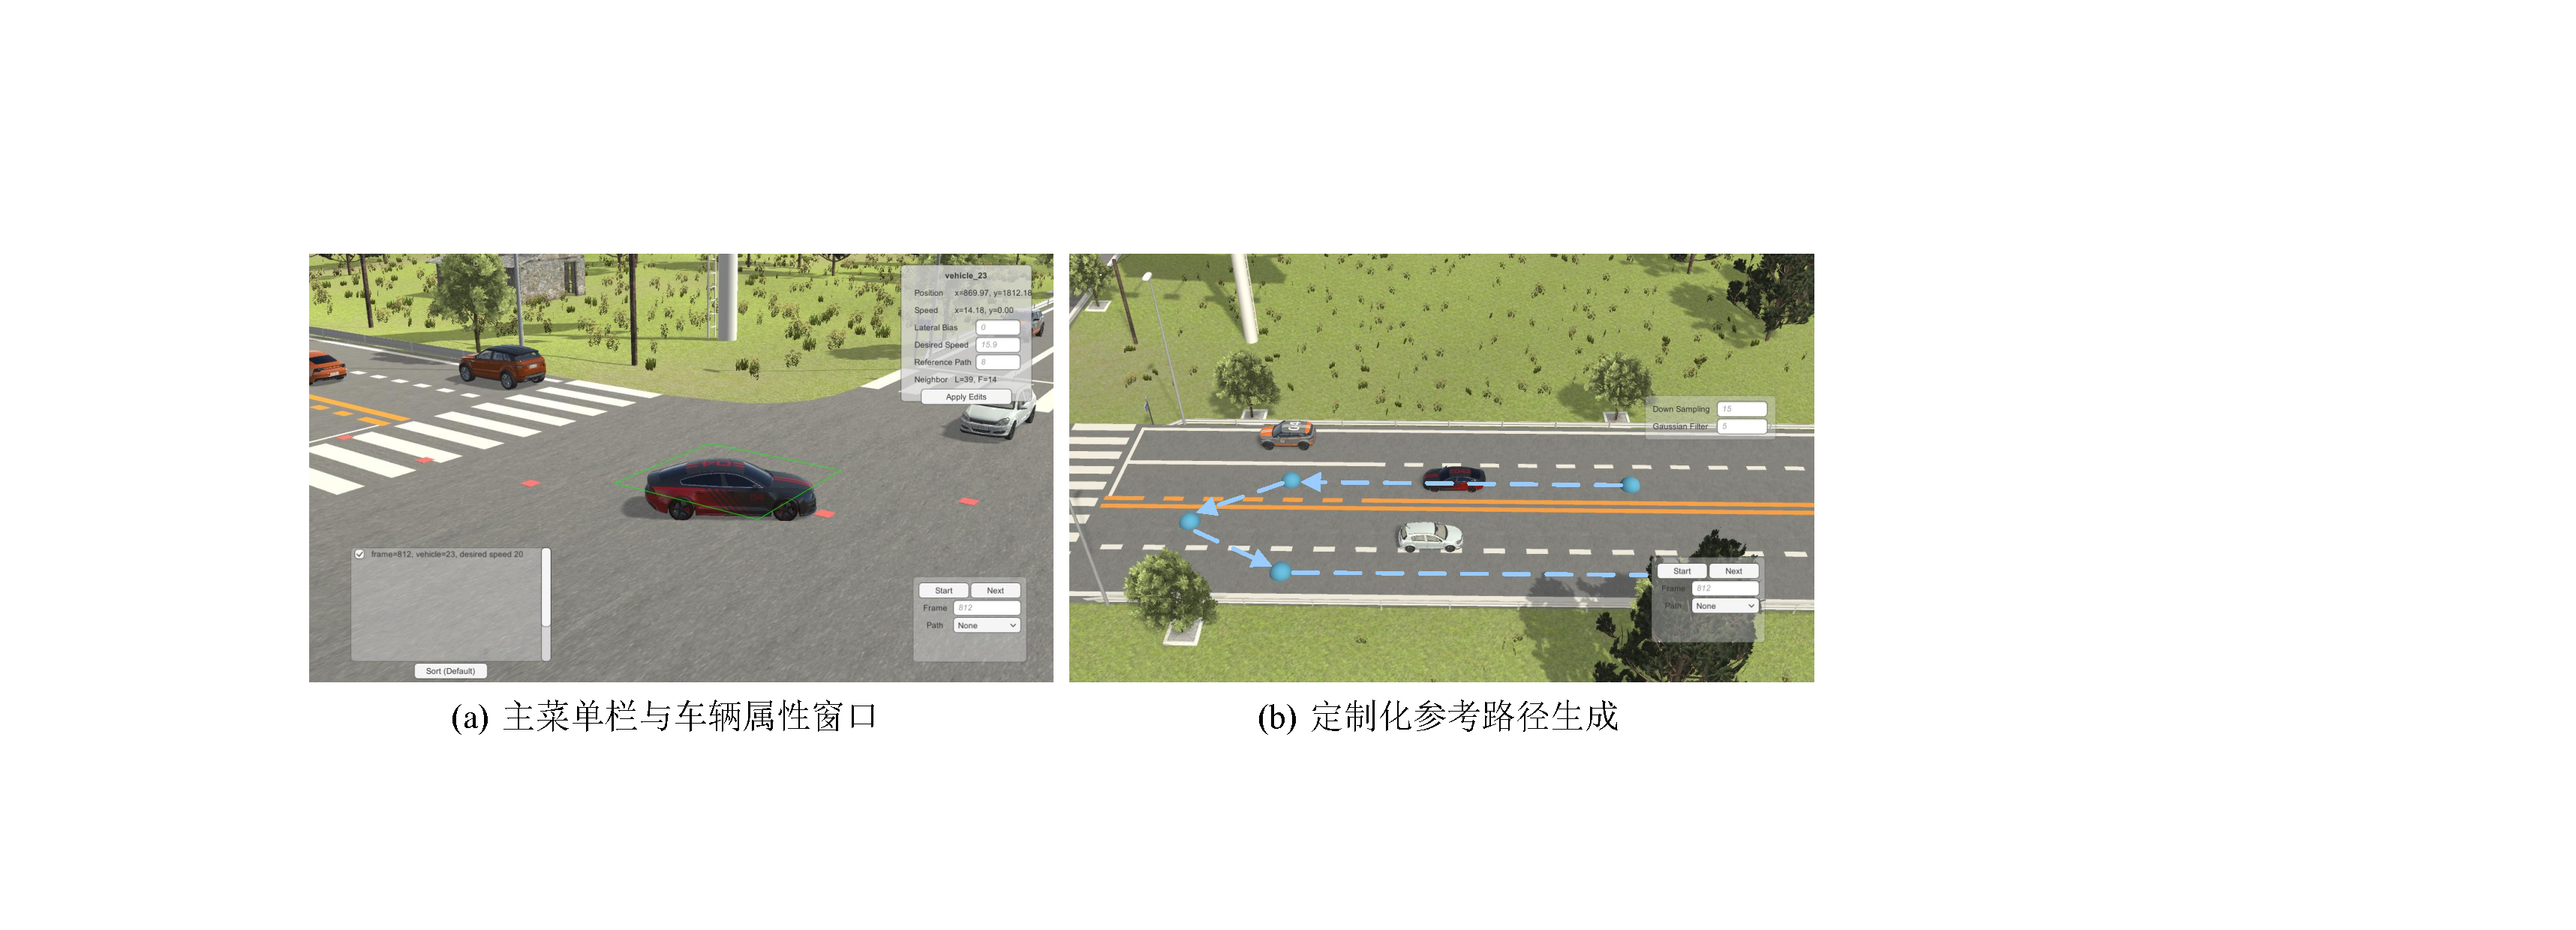
\includegraphics[width=\columnwidth]{figure/traedits/GUI v2.pdf}
%\caption[TraEITDS的用户图形界面]{TraEDITS的用户图形界面。 (a) 主菜单栏、编辑集合和车辆属性窗口,(b) 路径规划模式下点击的关键点,与后处理参数调整窗口。}
\caption[TraEITDS的用户图形界面]{
TraEITDS的用户图形界面
}
\label{fig:traedits_gui}
%\vspace{-0.45cm}
\end{figure}



\subsection{轨迹编辑案例}
\label{section:traedits_cases}

我们设计了四个案例用于展示用户通过TraEDITS对已有轨迹进行编辑的结果。


\begin{figure}[!tbh]
\centering
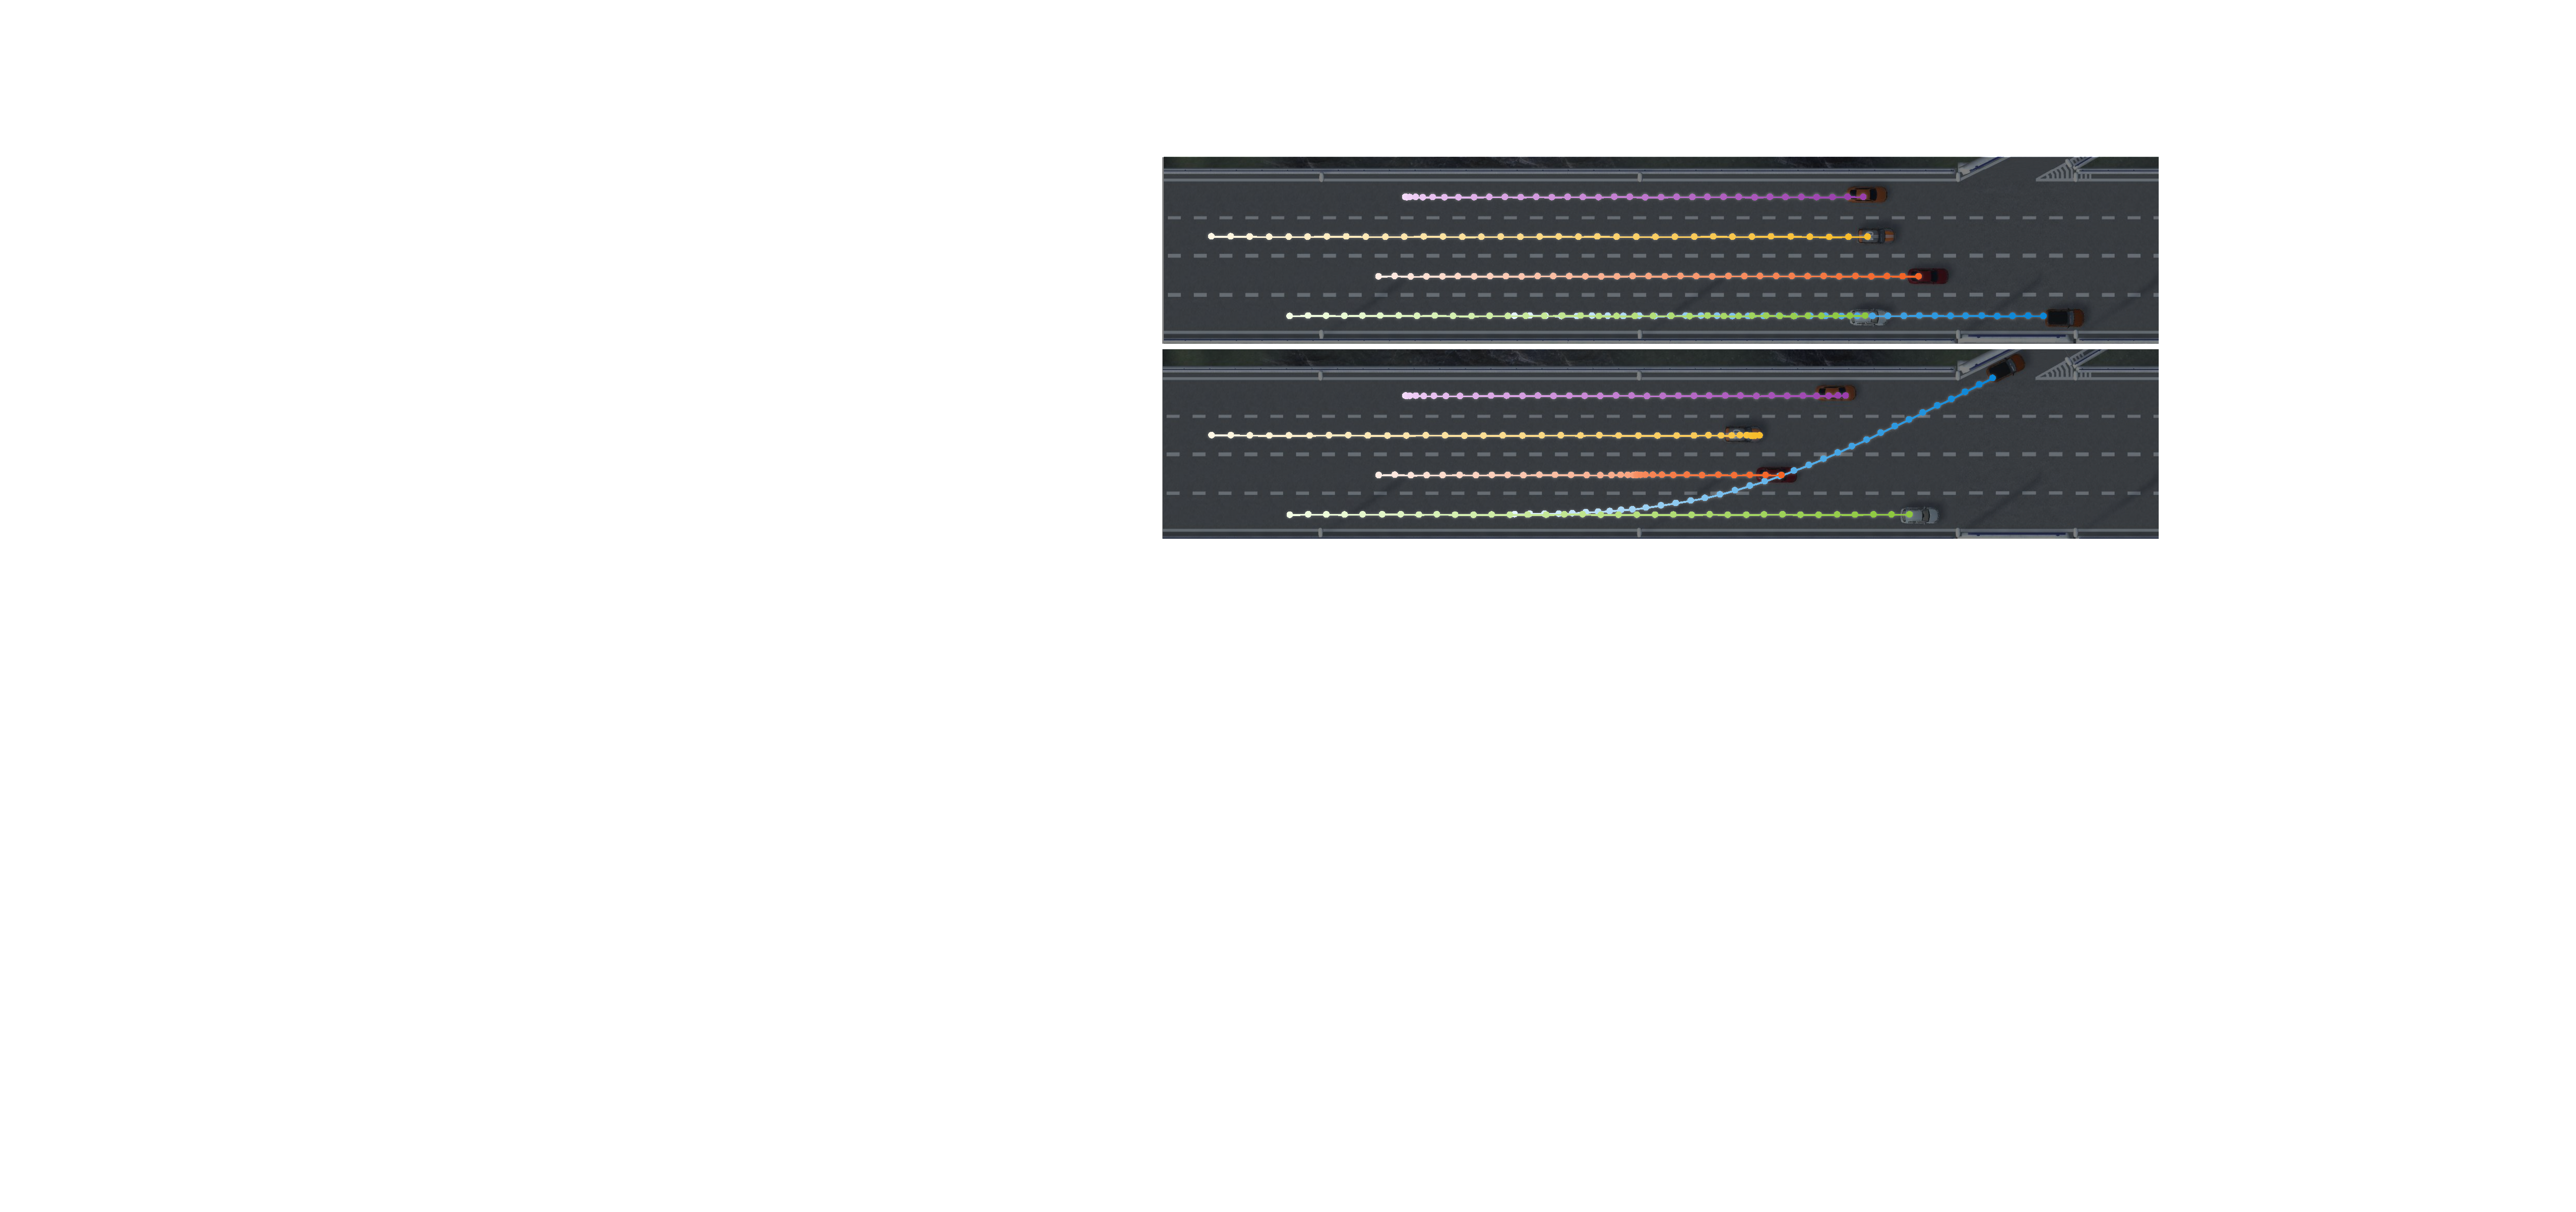
\includegraphics[width=\columnwidth]{figure/traedits/editing ramp 5.pdf}
%\caption[空旷高速路上急转弯编辑案例]{在包含匝道的空旷高速路上进行急转弯案例的原始轨迹(上)和编辑轨迹(下)。}
\caption[空旷高速路上急转弯编辑案例]{
空旷高速路上急转弯编辑案例
}
\label{fig:traedits_editramp}
\end{figure}

\begin{figure}[!tbh]
\centering
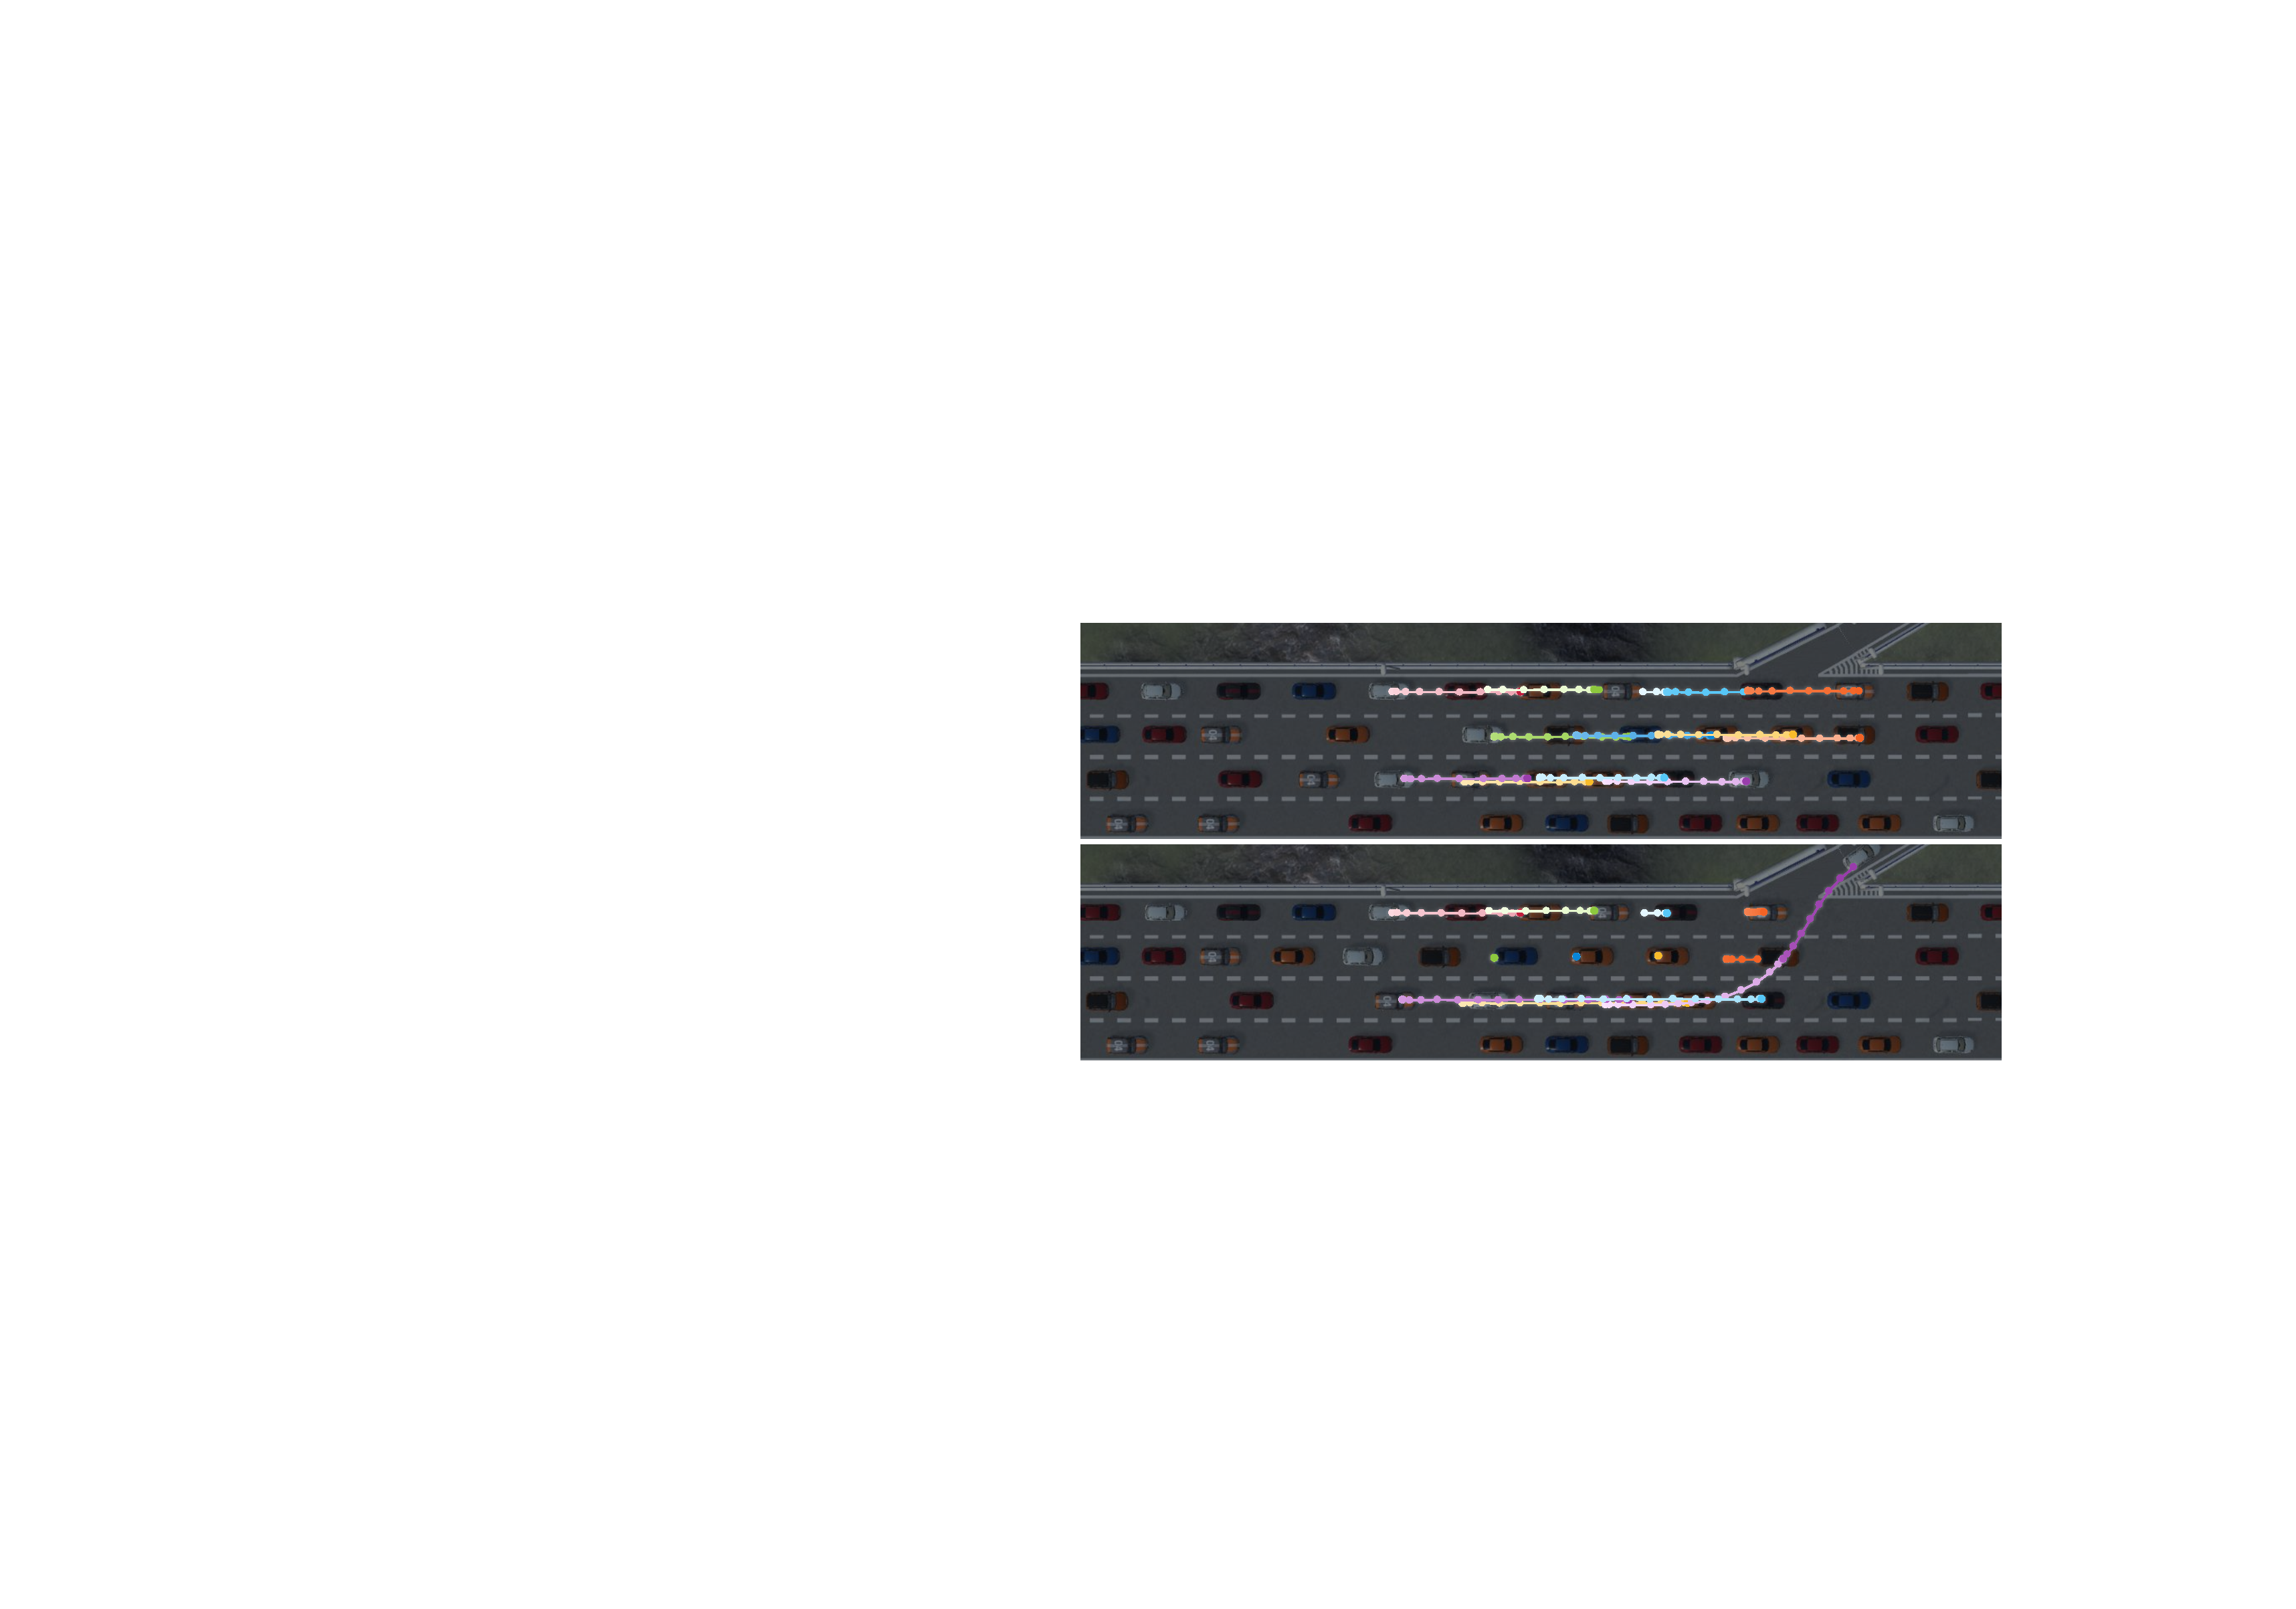
\includegraphics[width=\columnwidth]{figure/traedits/editing crowded 5.pdf}
%\caption[拥挤高速路上急转弯编辑案例]{在包含匝道的拥挤高速路上进行急转弯案例的原始轨迹(上)和编辑轨迹(下)。}
\caption[拥挤高速路上急转弯编辑案例]{
拥挤高速路上急转弯编辑案例
}
\label{fig:traedits_editcrowded}
\end{figure}

\begin{figure}[!tbh]
\centering
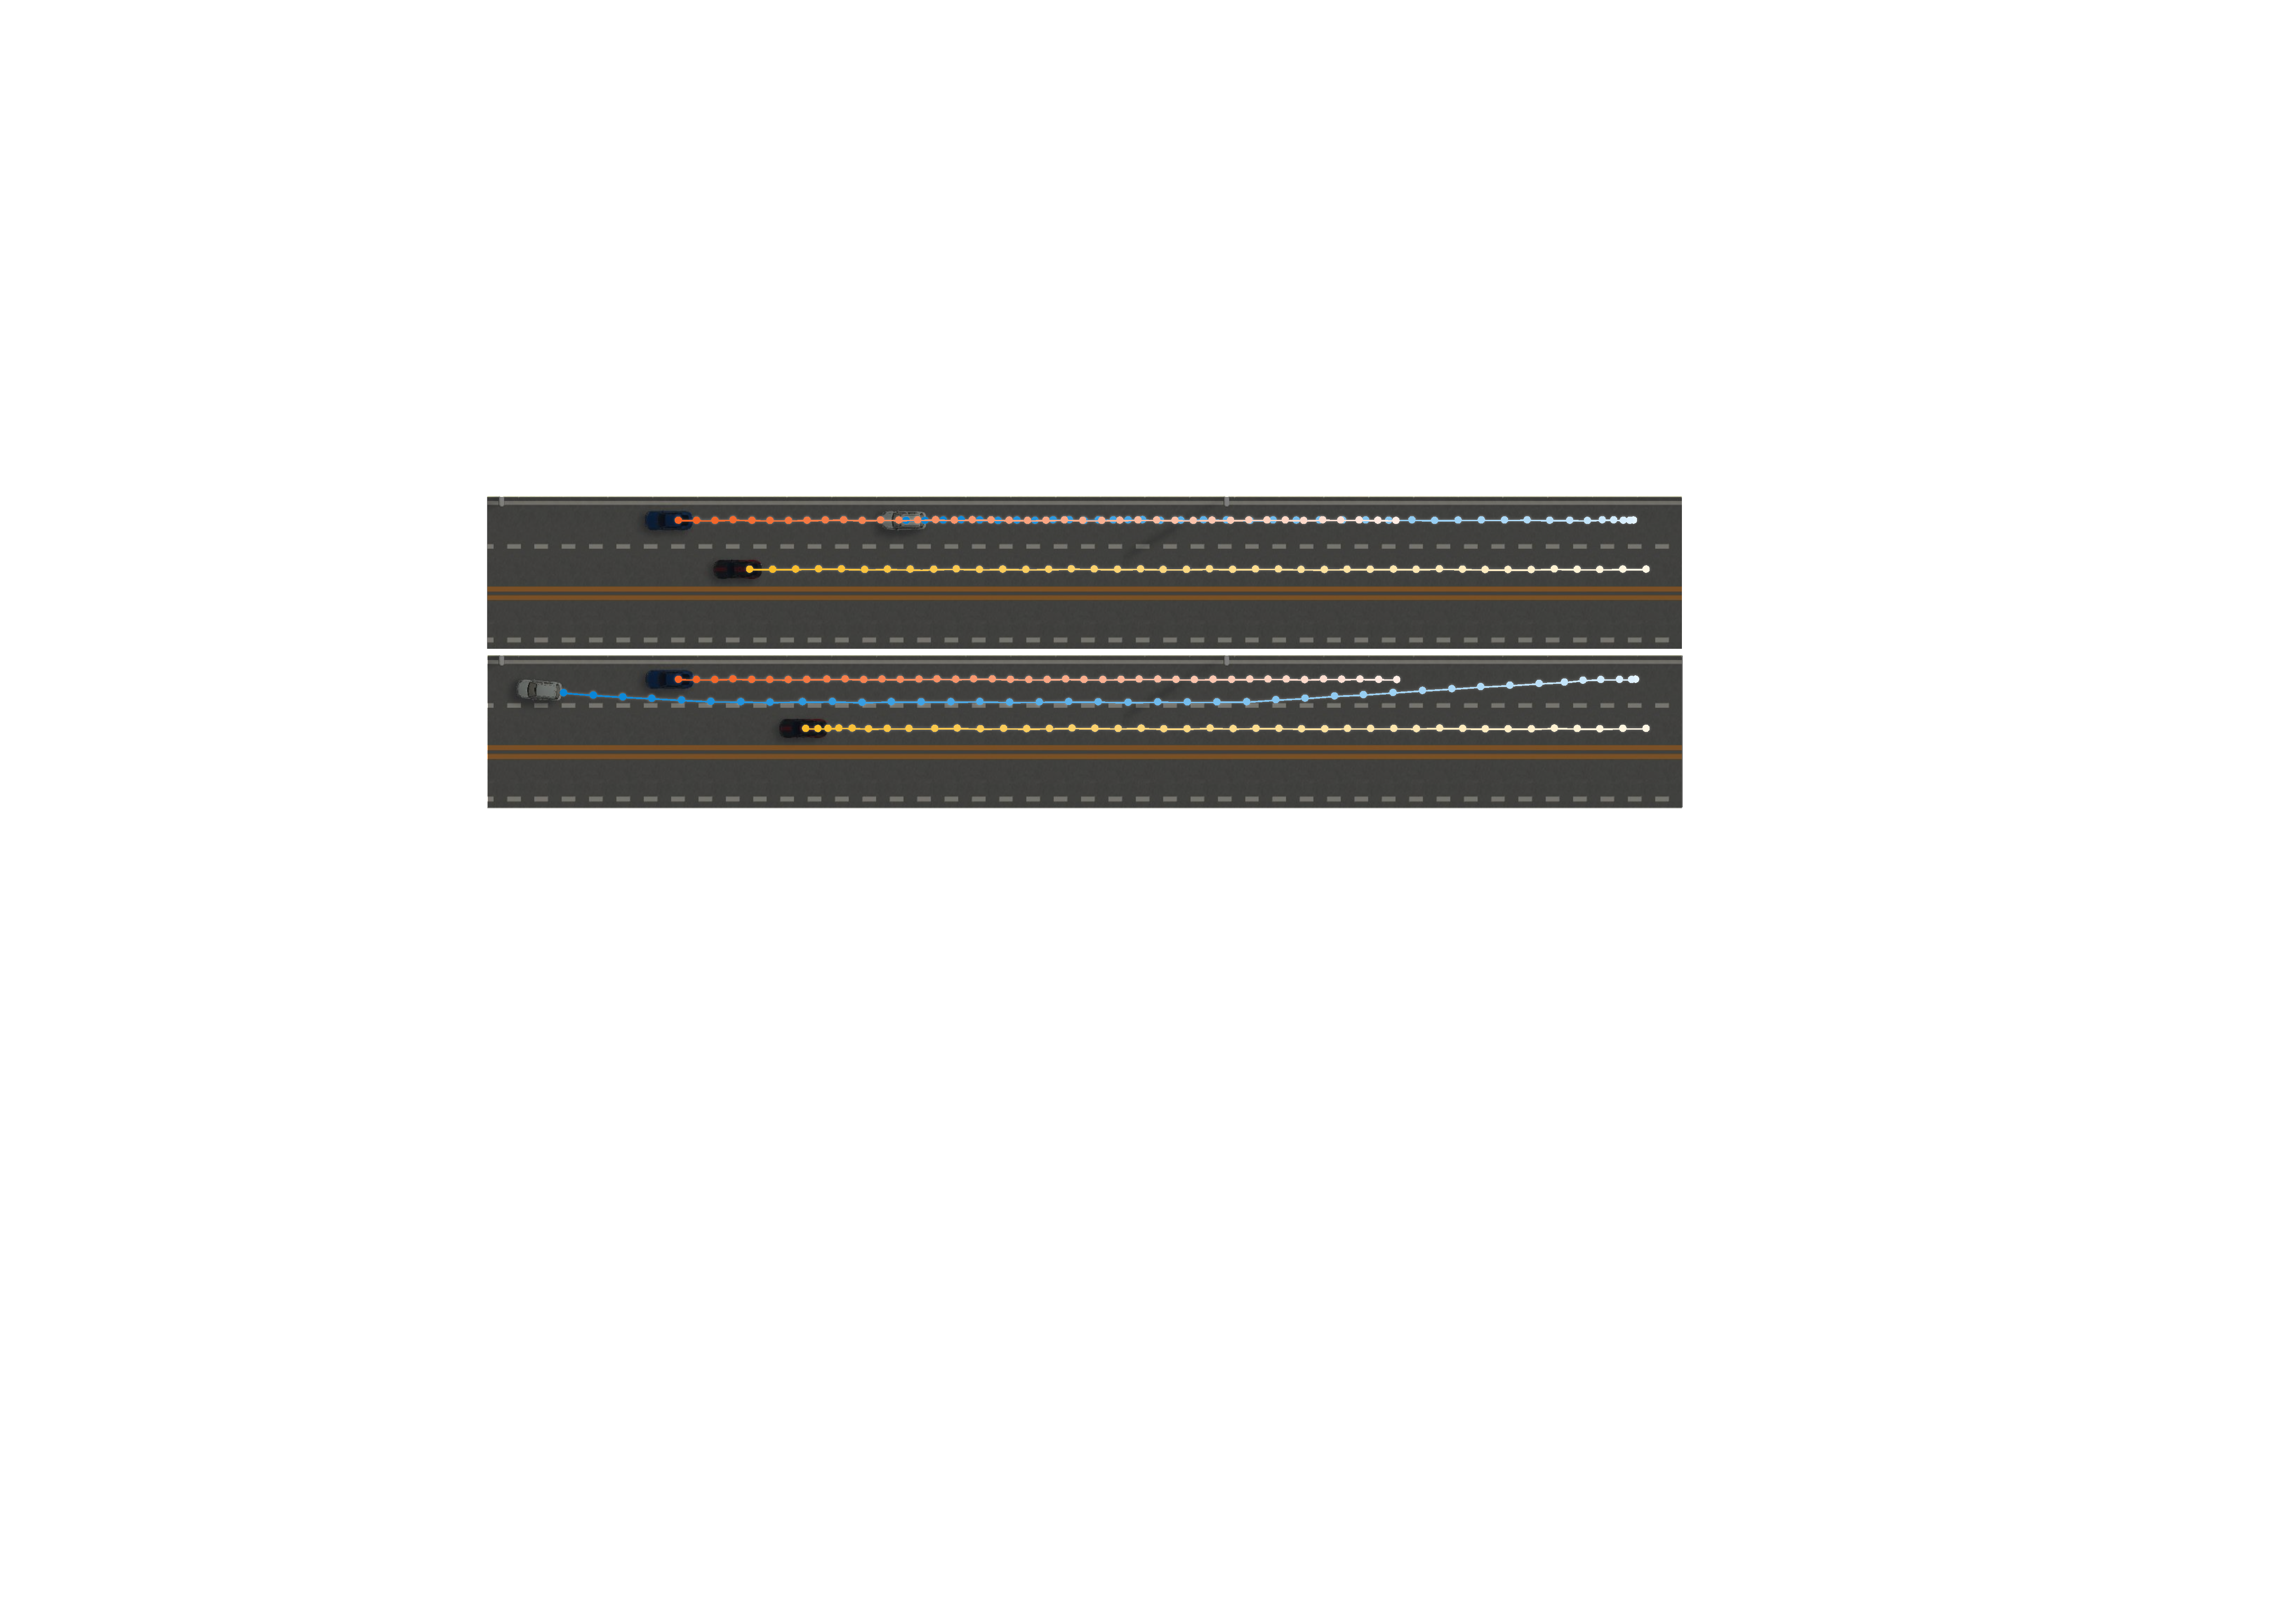
\includegraphics[width=\columnwidth]{figure/traedits/editing nudge 2.pdf}
%\caption[借道超车编辑案例]{借道超车案例的原始轨迹(上)和编辑轨迹(下)。}
\caption[借道超车编辑案例]{
借道超车编辑案例
}
\label{fig:traedits_editnudge}
\end{figure}

\begin{figure}[!tbh]
\centering
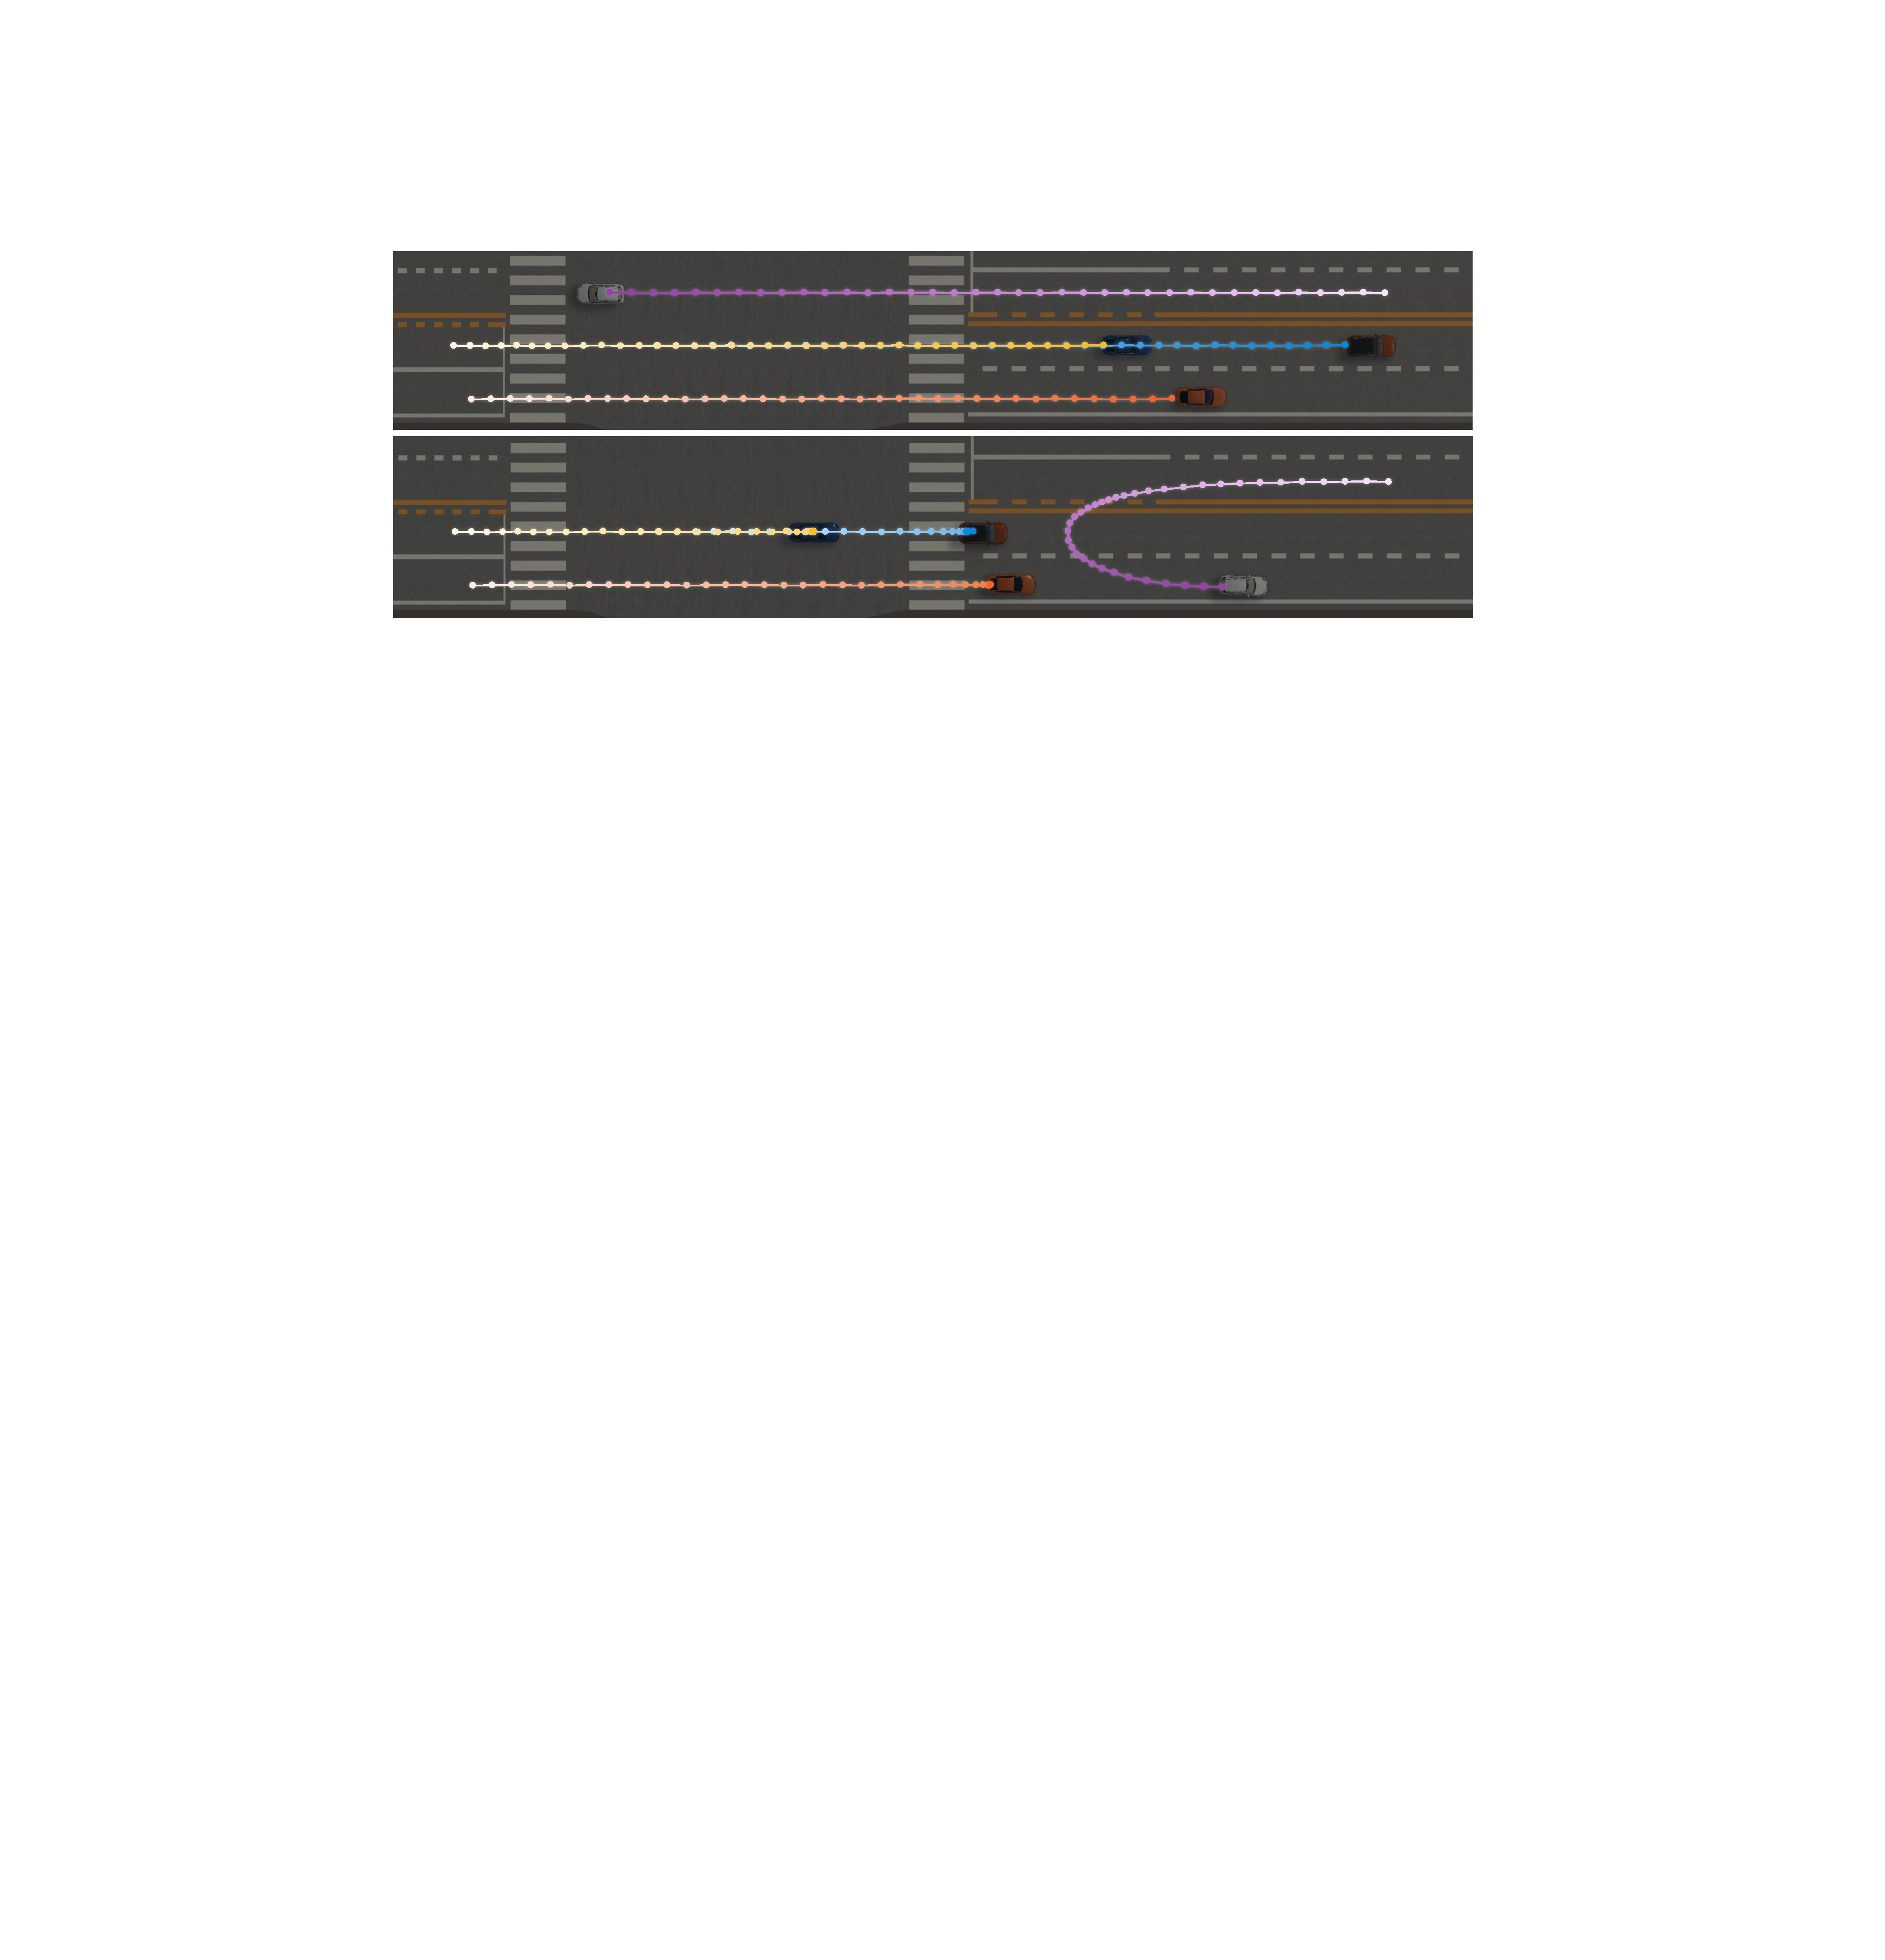
\includegraphics[width=\columnwidth]{figure/traedits/editing u-turn 5.pdf}
%\caption[U型掉头编辑案例]{U型掉头案例的原始轨迹(上)和编辑轨迹(下)。}
\caption[U型掉头编辑案例]{
U型掉头编辑案例
}
\label{fig:traedits_edituturn}
\end{figure}




前两个案例在包含匝道的高速公路场景中生成。在第一个案例中,我们手动定义了一条参考路径,其在一个很短的距离内从最远的车道横跨四车道后进入了匝道。我们将这条参考路径赋予原本在离匝道最远的车道上行驶的一辆车,使其的运动像是在快要错过匝道时突然急转弯跨多车道后驶入匝道,如图~\ref{fig:traedits_editramp}所示。在第二个案例中,我们在相同的道路但是拥挤的交通环境中也生成了类似的跨多车道急转弯的车辆行为。原先车辆在离匝道最远的道路上排队等候,编辑后则在短距离内穿过了其他车道的所有车辆,实现跨多车道,最终进入了匝道离开主路,如图~\ref{fig:traedits_editcrowded}所示。


后两个案例在包含十字路口的场景中生成。在第三个案例中,我们让一辆在当前车道和邻车道均被前车堵塞的车辆稍稍偏离了参考路径,使其在压虚线的情况下成功借道并超越两辆前车,如图~\ref{fig:traedits_editnudge}所示。在第四个案例中,我们自定义了一条参考路径使车辆在十字路口处进行U型掉头后使入相反方向的车道中,车辆能够在过急弯道的时候实现先缓慢降低速度后平稳恢复原始状态,且来车均能减速并等待其完成掉头,如图~\ref{fig:traedits_edituturn}所示。

上述案例展示出TraEDITS框架拥有生成原先方法难以生成或是先有数据集中很少被采集到的非常规交通行为,这些行为在三维场景中可视化后可以应用于自动驾驶虚拟道路测试或数据增广等目的,如图~\ref{fig:traedits_firstperson}为U型掉头案例在Unity3D中可视化并从来车驾驶员角度观察的截图。

\begin{figure}[!tbh]
\centering
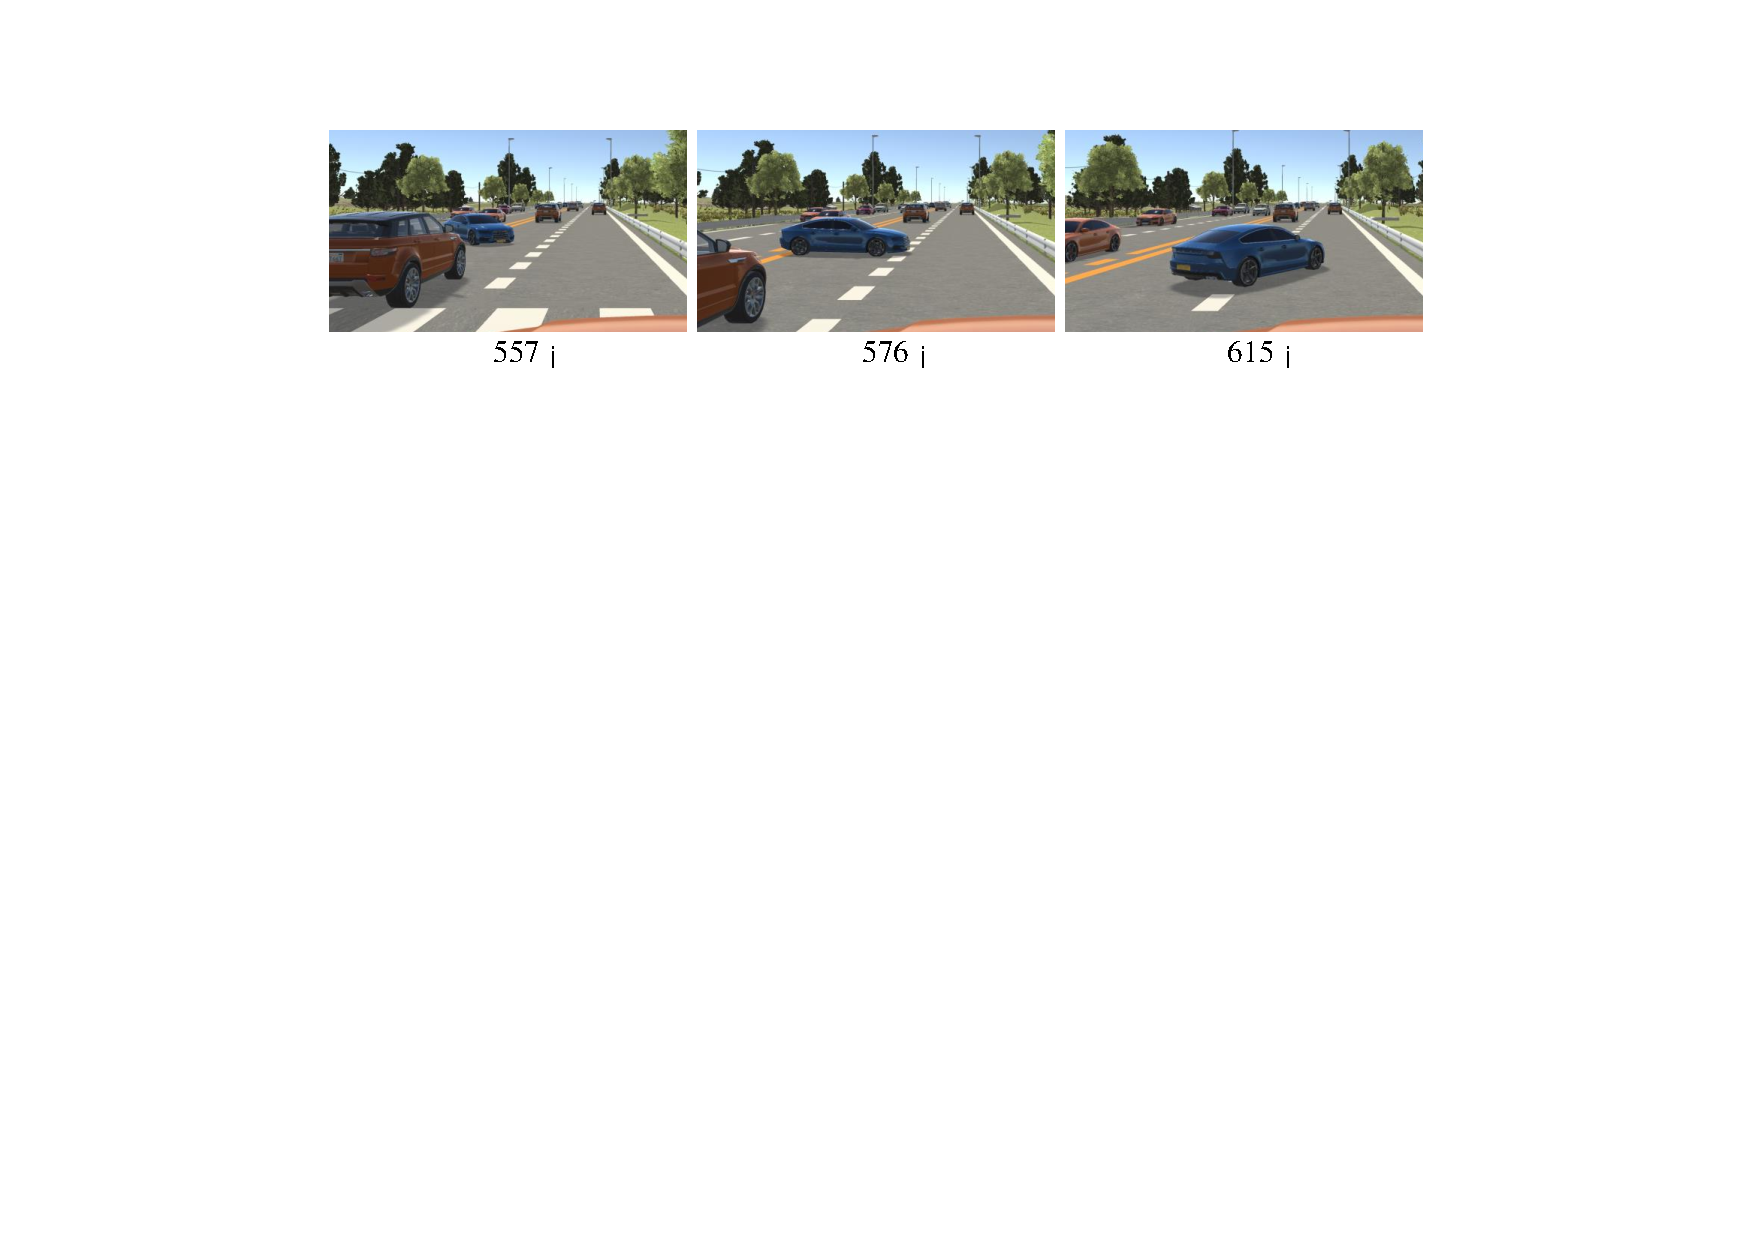
\includegraphics[width=0.9\columnwidth]{figure/traedits/first person view 2_cn.pdf}
%\caption[驾驶员视角的U型掉头]{在Unity3D中可视化U型掉头案例,并从来车驾驶员视角观察的截图。 }
\caption[邻车驾驶员视角的U型掉头结果]{
邻车驾驶员视角的U型掉头结果
}
\label{fig:traedits_firstperson}
\end{figure}


\subsection{性能分析}
\label{section:traedits_performance}

\begin{figure}[!tbh]
%\setlength{\abovecaptionskip}{-0.05cm} 
%\setlength{\belowcaptionskip}{-0.2cm}
\centering
    \centering
    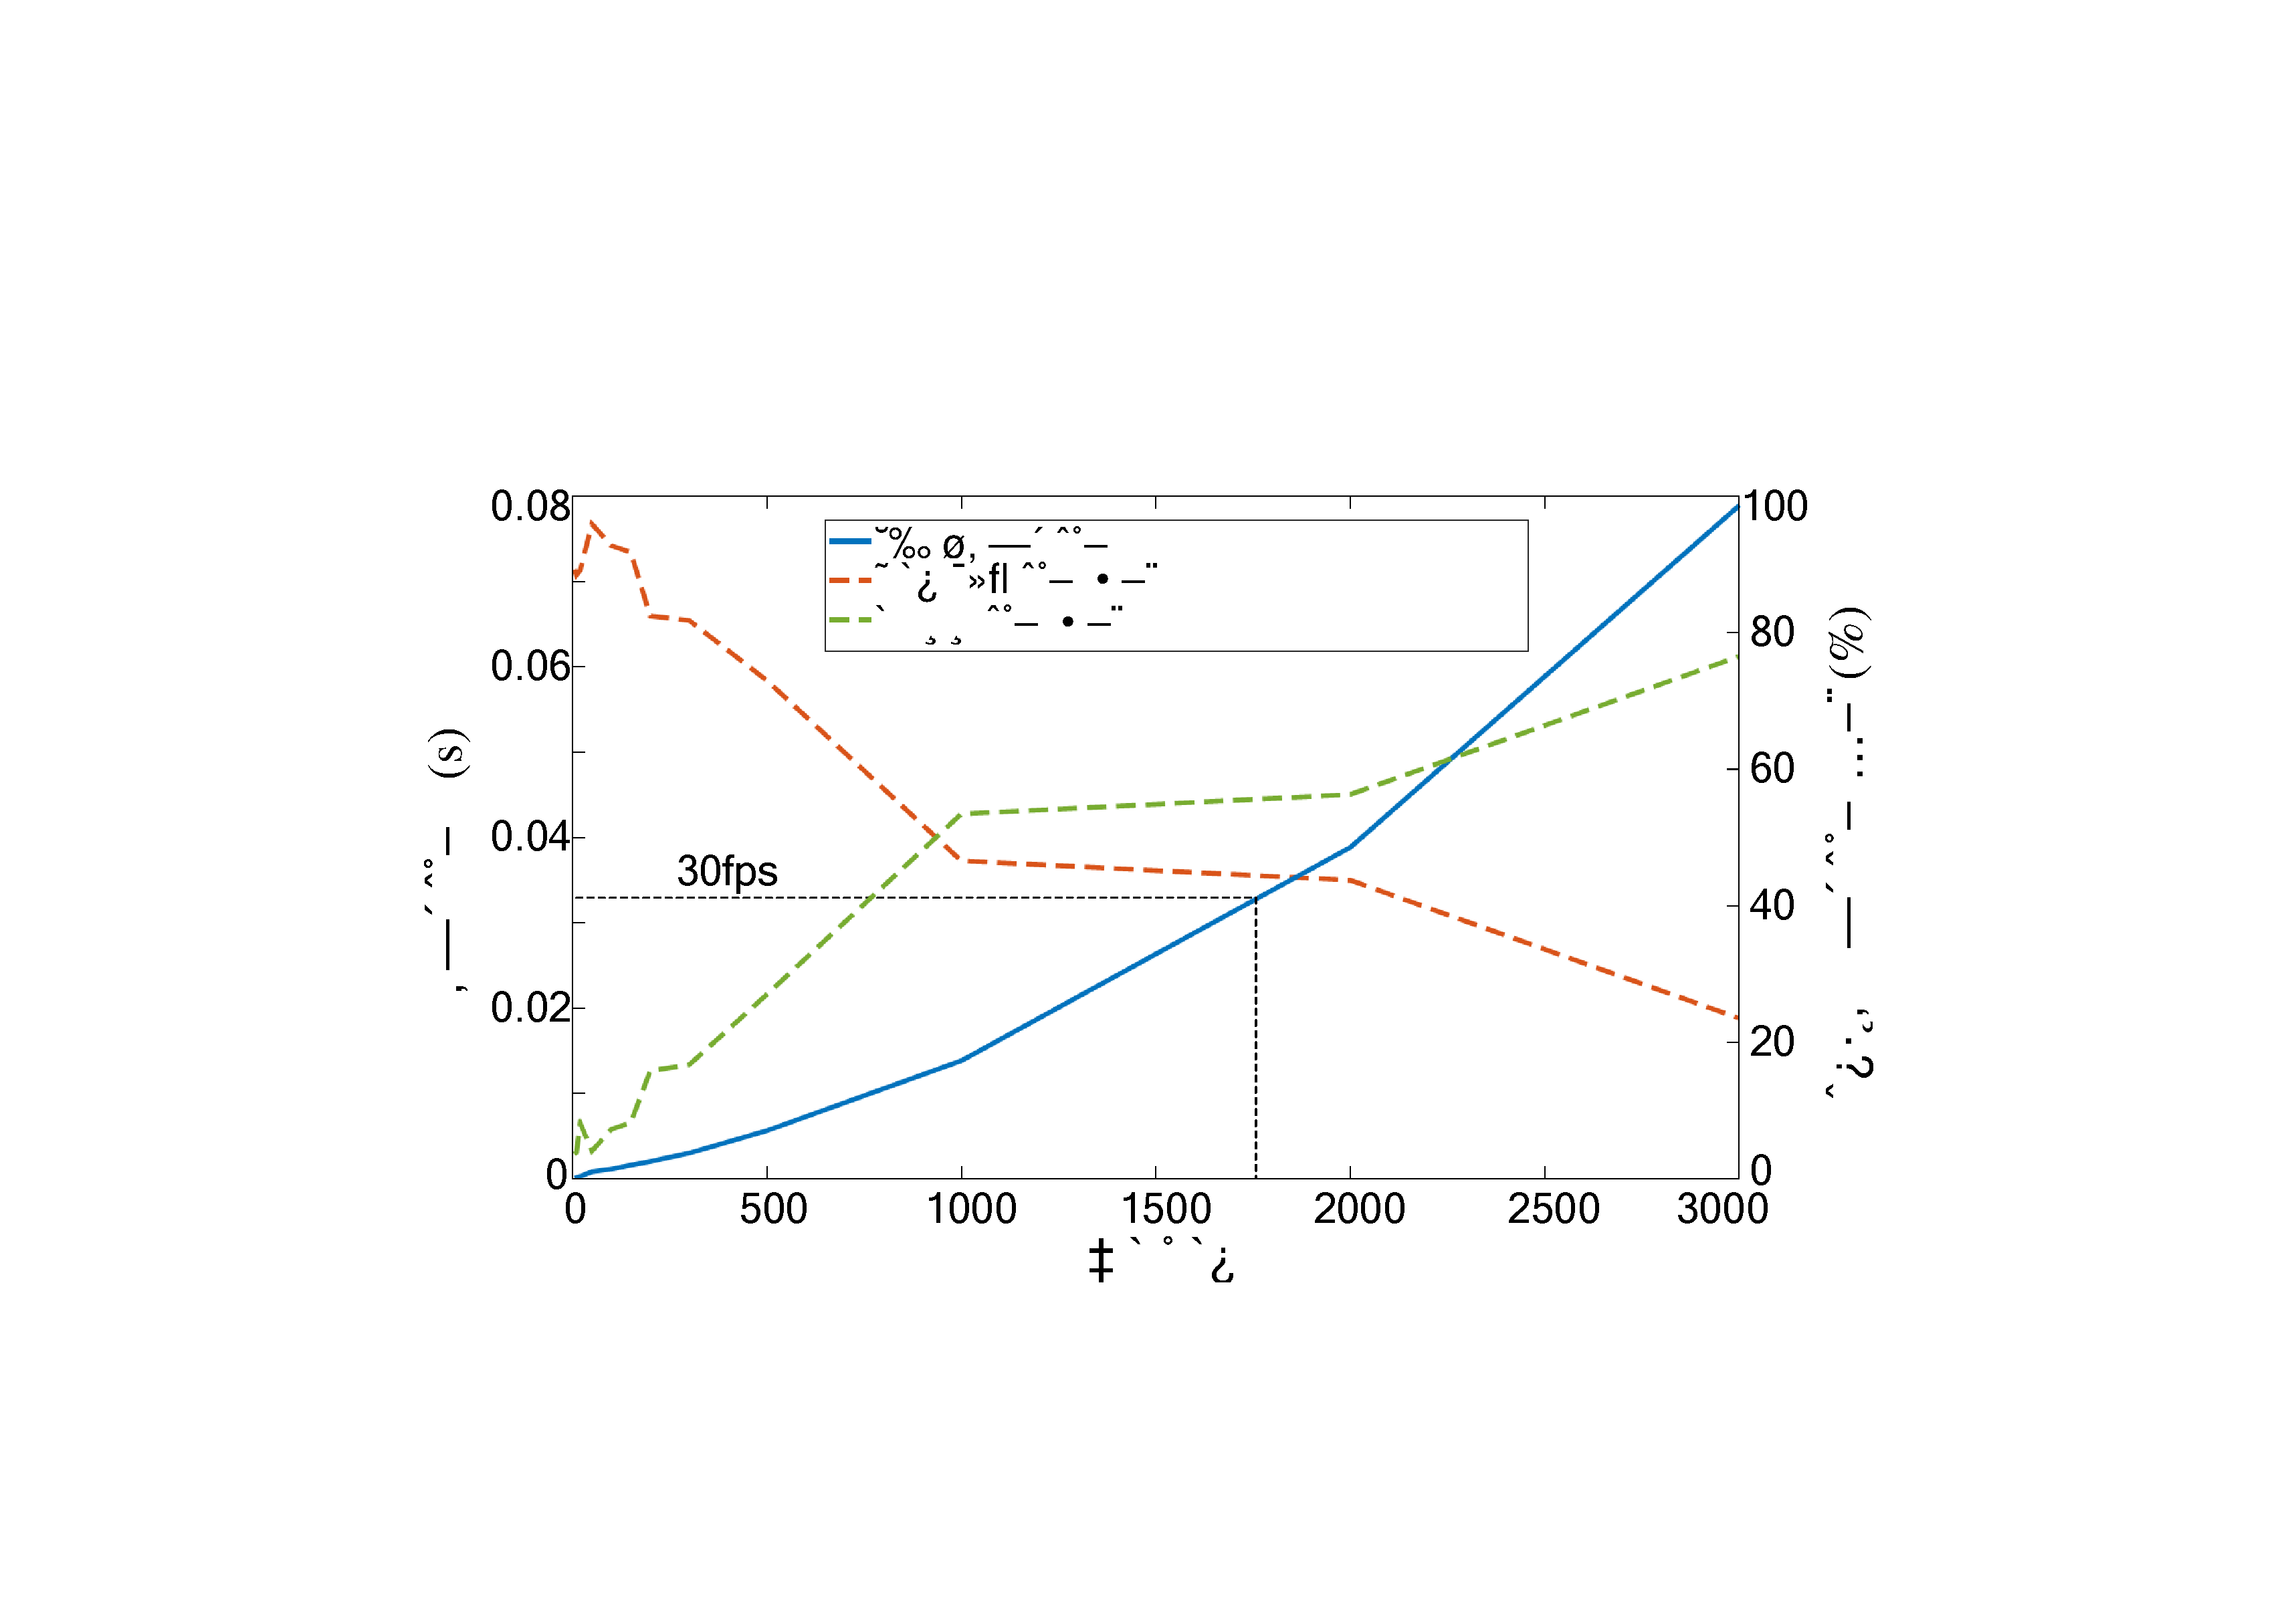
\includegraphics[width=0.78\columnwidth]{figure/traedits/performance simulation 4_cn.pdf}
    %\caption[TraEDITS框架交通仿真模块运行效率]{TraEDITS框架中交通仿真模块的运行效率。基于车辆状态的并行更新策略,我们不断更改场景中车辆的数量,并统计了更新一帧所使用的时间(秒),以及其中能量最小化过程和邻车搜索过程所占的时间比例。}
    \caption[TraEDITS框架交通仿真模块运行效率]{TraEDITS框架交通仿真模块运行效率}
    %Performance of the traffic simulation module. We show average update time (s) with parallel implementation, time percentage of energy optimization and neighbors search per frame over different numbers of vehicles. }
    \label{fig:traedits_simperform}
%\vspace{-0.45cm}
\end{figure}


为了测试TraEDITS交通仿真模块的运行效率,我们在包含不同数量车辆的场景中统计了TraEDITS的更新用时。如图~\ref{fig:traedits_simperform}所示,基于车辆状态的并行更新策略,我们不断更改场景中车辆的数量,并统计了更新一帧所使用的时间(秒),发现一帧的更新时间随着车辆数量的增加基本呈线性增长,在测试场景中存在1800辆车时仍能保持30fps的更新帧率。我们进一步统计了仿真方法中能量最小化过程和邻车搜索过程所占的时间比例。显然,随着车辆数量的增加,邻车搜索所用的时间占比将增加,能量最小化所用的时间占比随之下降。事实上对一辆车而言,更新其状态的能量最小化过程所用的计算时间几乎是保持不变的,但当交通环境越来越拥挤时,其邻车数量会增多,因此在计算碰撞避免时判断其邻车集合所用的时间也会增加。



为了测试TraEDITS全局规划模块的参考路径生成效率,我们通过随机指定不同个数的关键点、生成不同长度的参考路径,来统计对比路径生成所用的总时间、启发式搜索的搜索步数和最终路径中车道中心线的所占的比例,如表~\ref{tab:traedits_planperform}所示。首先,保持路径的总长度不变,我们统计了给定不同个数关键点时路径规划总时间的变化;其次,在保持给定关键点个数为5时,我们统计了不同路径总长度下规划总时间的变化。显然,当关键点个数增加或减少路径总长度时,规划路径所需的总时间会下降。当只给定两个关键点来规划一条很长的路径时,这两个点就扮演了整个启发式搜索流程的起点和终点,启发式搜索的步数会由于大量的试错而急剧增长。另外值得注意的是,实验中全局规划模块搜索得到的路径车道线中心占比部分均超过了70\%,这验证了我们的启发式函数~\ref{eq:traedits_planingheuristic}是有效的,而这一比例在指定关键点个数增加或路径总长度减少时下降。

\begin{table}[!tbh]
%\setlength{\abovecaptionskip}{-0.01cm} 
\setlength{\belowcaptionskip}{.4cm}
\centering
%\small
%\resizebox{\columnwidth}{!}
%{
\renewcommand\arraystretch{2.0}
%\caption[TraEDITS框架全局规划模块路径生成效率]{TraEDITS框架中全局规划模块的路径生成效率。我们分别统计了在不同个数关键点和不同路径长度(英尺)时,生成路径时启发式搜索的搜索步数,生成的路径落在车道中心线部分占路径总长度的比例,以及规划所需的总时间(秒)。}
\caption[TraEDITS框架全局规划模块路径生成效率]{TraEDITS框架中全局规划模块的路径生成效率}
\begin{tabular}{|c|c|c|c|c|}
\hline
\begin{tabular}[c]{@{}c@{}}关键点个数\end{tabular} &
  \begin{tabular}[c]{@{}c@{}}路径总长度 \\(米)\end{tabular} &
  \begin{tabular}[c]{@{}c@{}}启发式搜索步数\end{tabular} &
  \begin{tabular}[c]{@{}c@{}}车道中心线部分占比\end{tabular} &
  \begin{tabular}[c]{@{}c@{}}规划总时间 \\ (秒)\end{tabular} \\ \hline
2                  & 783.7 & 222,066 & 99.47\% & 25.61 \\ \hline
3                  & 783.0 & 142,026 & 99.03\% & 8.44  \\ \hline
\multirow{3}{*}{5} & 786.1 & 31,186  & 97.81\% & 1.08  \\ \cline{2-5}
                   & 417.9 & 5,867   & 89.33\% & 0.21  \\ \cline{2-5}
                   & 219.8  & 1,595   & 78.50\% & 0.11  \\ \hline %\\ \cline{2-5}
%                   & 422.28  & 1232   & 67.71\% & 0.07  \\ \hline
10                 & 781.3 & 7,657   & 90.01\% & 0.20 \\ \hline
\end{tabular}
\label{tab:traedits_planperform}
\end{table}




\subsection{用户调查}
\label{section:traedits_userstudy}

我们设计了两场用户调查,第一场用于验证TraEDITS的易用性,第二场用于验证TraEDITS的轨迹编辑结果的真实感。两场用户调查的参与者均为18人,其中13人为男性,其余5人为女性。

\textbf{易用性验证:}在第一场用户调查中,参与者被要求使用TraEDITS轨迹编辑框架完成如下三个任务:

\begin{enumerate}
    \item 在指定车辆原先被另一辆速度较慢的前车阻挡的情况下,使其成功超越前车。

    \item 在指定车辆原先直行通过十字路口的情况下,使其在进入路口前U型掉头并驶入对向车道。

    \item 在十字路口每个方向有15辆来车且无信号灯控制的情况下,使所有车辆安全通过路口。
\end{enumerate}

完成上述所有任务后,参与者被要求填写一份NASA任务负荷指数量表(NASA Task Load Index)~\cite{hart1988development, hart2006nasa},包含精神负荷(mental demand)、体力负荷(physical demand)、时间消耗(temporal demand)、完成度(performance)、努力程度(effort)和受挫程度(frustration)六个维度。参与者需要基于完成任务的过程,对上述六个维度从1到5进行打分,分值越高代表负荷越高、耗时越长、完成度越高或努力和受挫程度越高。此外,量表最后还有三句陈述性总结,参与者需要对其分别从1到5进行认可度的打分,分值越高代表越同意总结所述观点。

%\begin{figure}[!tbh]
%    \centering
%    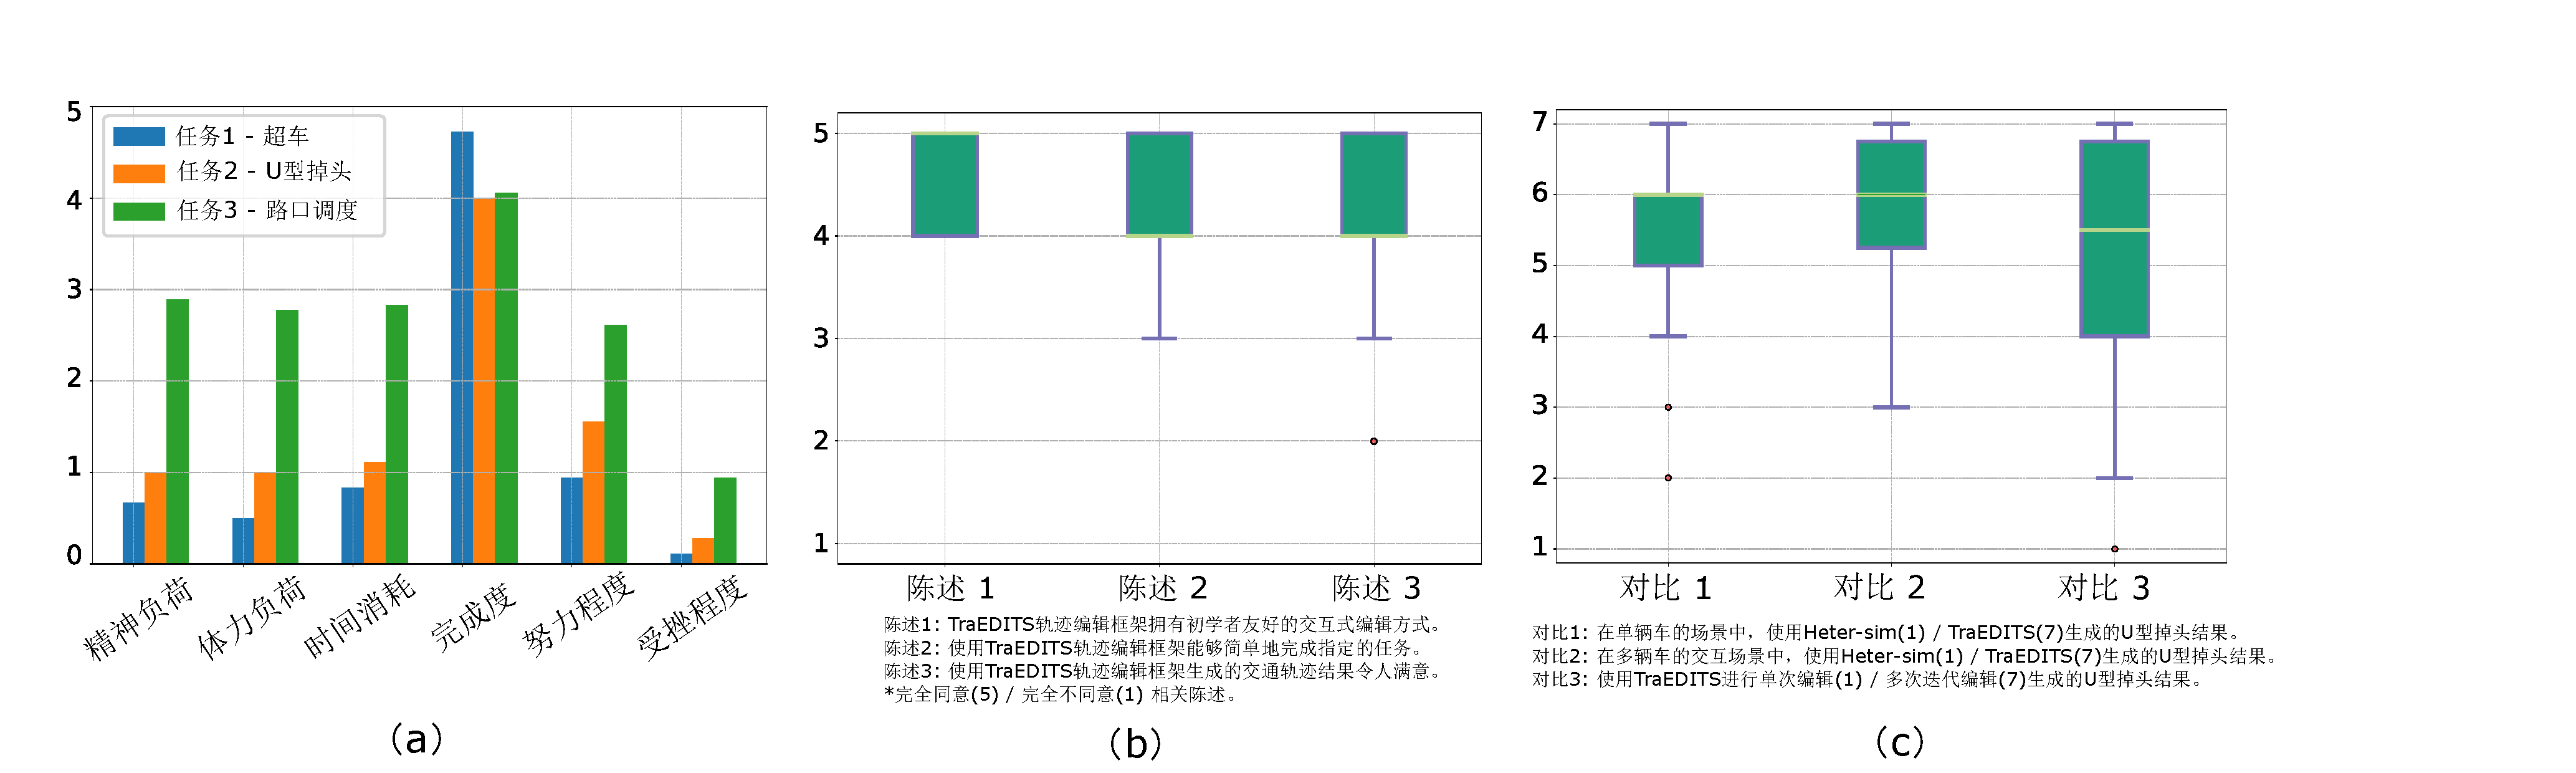
\includegraphics[width=\textwidth]{figure/traedits/userstudy combine cn.pdf}
    %\caption[TraEDITS用户调查结果]{(a) 参与者使用TraEDITS轨迹编辑框架完成指定任务后,NASA任务负荷指数量表的平均打分结果。(b) 参与者对三句陈述性总结的认可度打分结果。 (c) 参与者对三对对比实验的打分结果。 }
%    \caption[TraEDITS用户调查结果统计]{
%    TraEDITS用户调查结果统计
%    }
%    \label{fig:traedits_userstudy}
%\end{figure}

\begin{figure}[!htb]
\centering
    \begin{subfigure}{0.5\textwidth}
        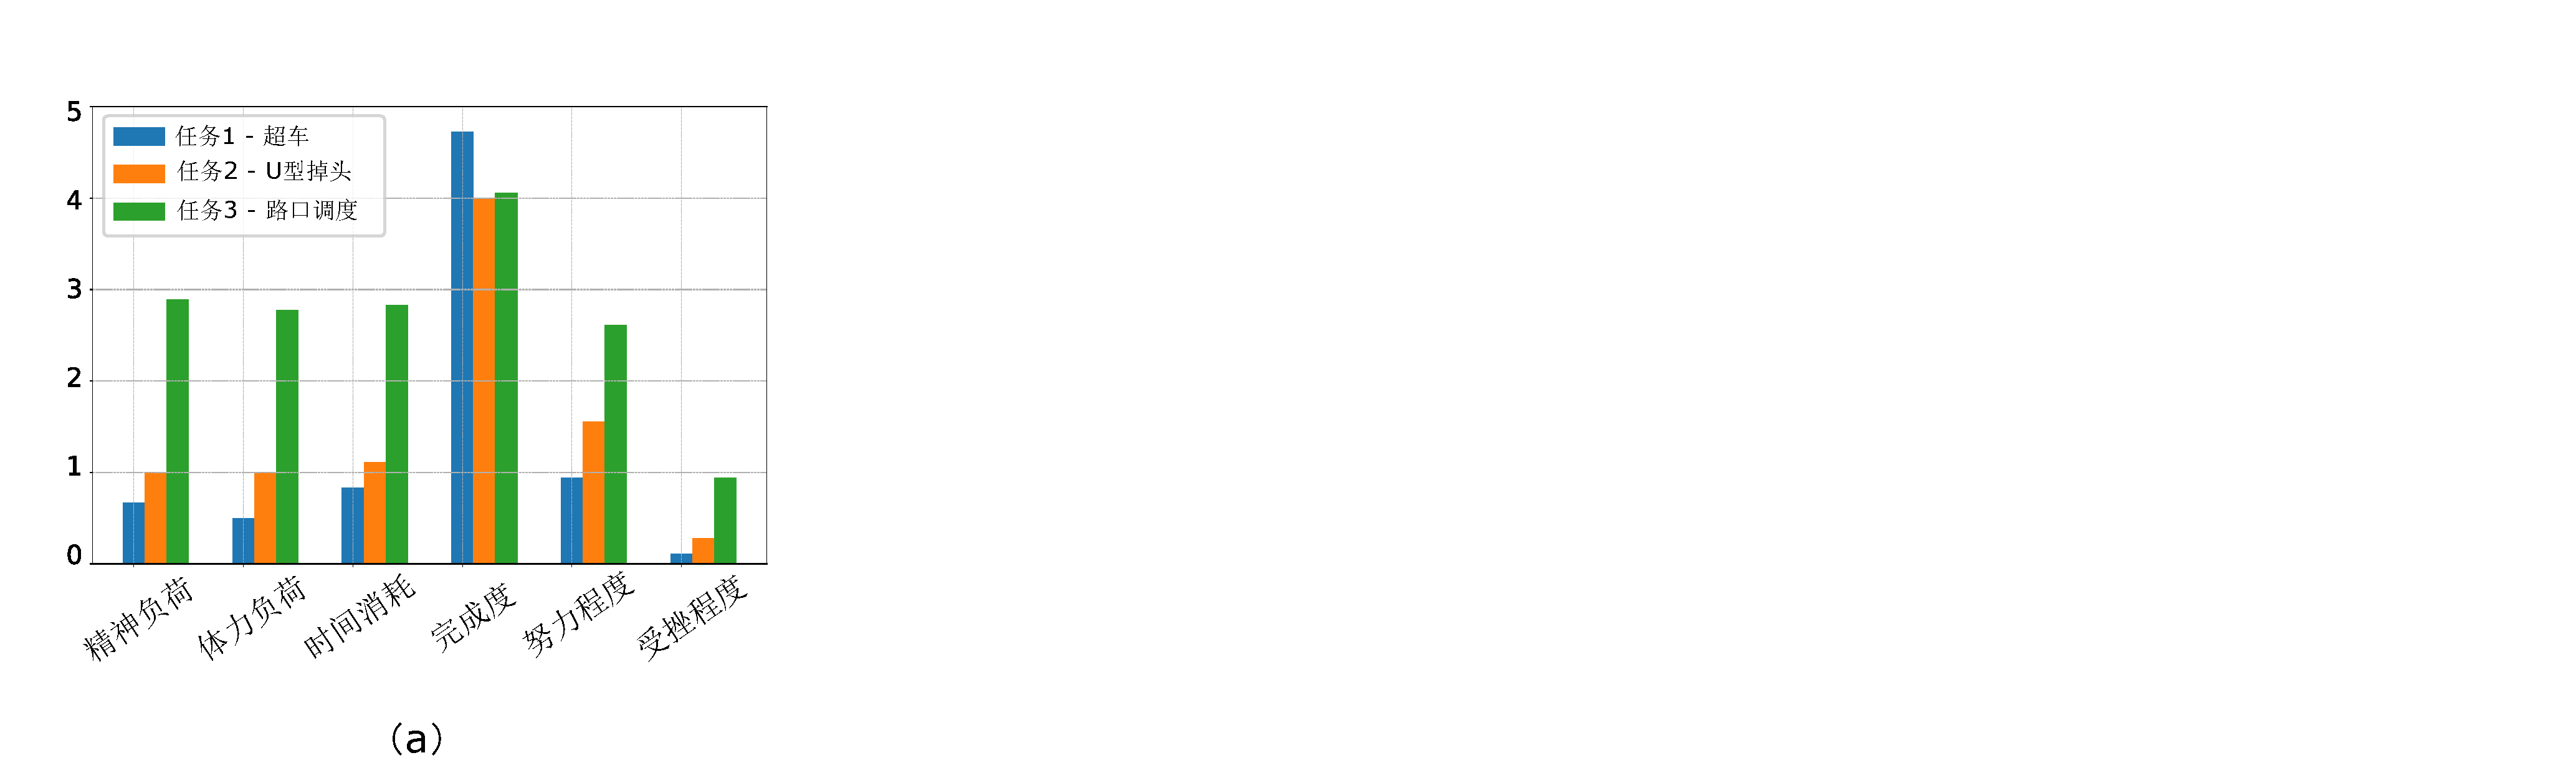
\includegraphics[width=\textwidth]{figure/traedits/userstudy cn 1.pdf}
        %\caption{First sub-figure caption.}
        %\label{fig:sub1}
    \end{subfigure}
    \\
    \begin{subfigure}{\textwidth}
        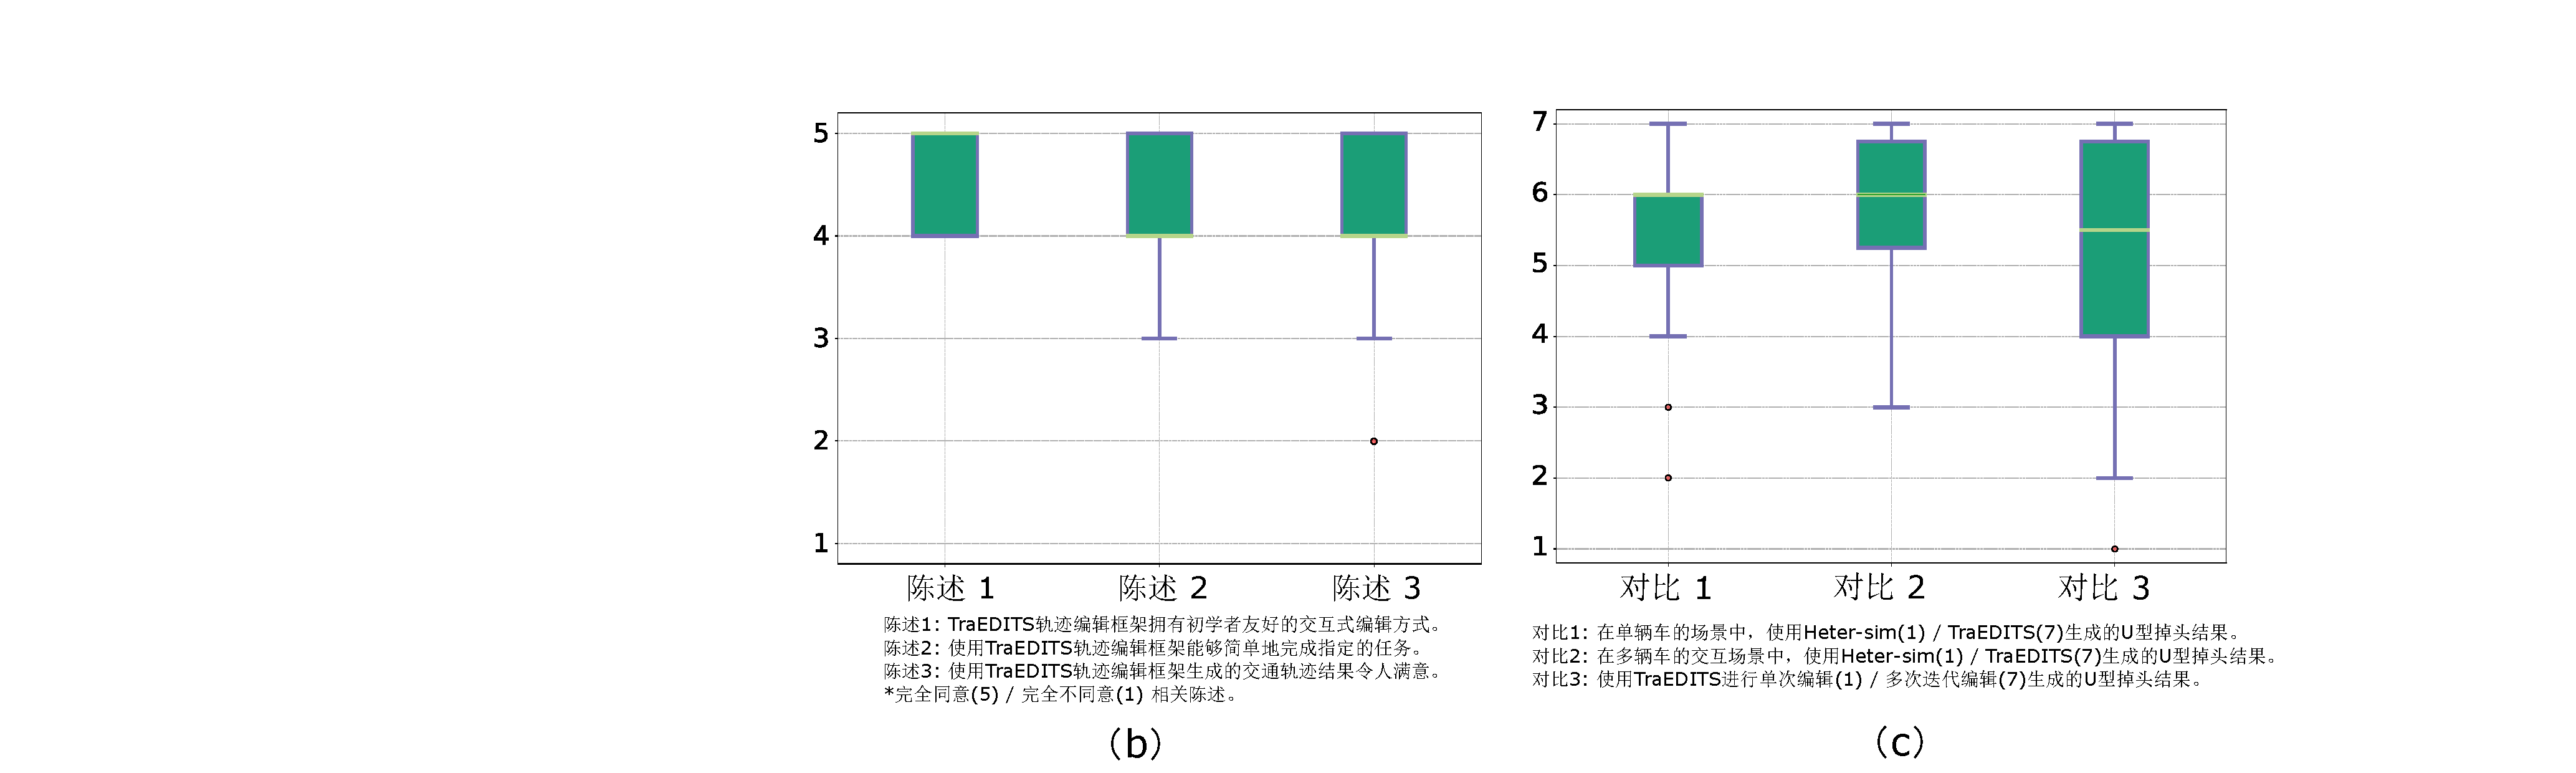
\includegraphics[width=\textwidth]{figure/traedits/userstudy cn 4.pdf}
    \end{subfigure}
    
    \caption[TraEDITS用户调查结果统计]{
    TraEDITS用户调查结果统计
    }
    \label{fig:traedits_userstudy}
\end{figure}


图~\ref{fig:traedits_userstudy}(a)中展示的是参与者使用TraEDITS完成指定任务后对NASA任务负荷指数量表的平均打分结果。除了第三个任务之外,其余两个任务参与者在精神负荷、体力负荷、时间消耗、努力程度和受挫程度五个维度上均小于2分,而使用TraEDITS完成三个任务的完成度均高于4分。这是因为在第三个任务中需要编辑的车辆数量更多,整个仿真持续的时间更长,因此用户需要消耗的精力也比其他两个任务更多。总体来说,使用TraEITDS进行交互式交通轨迹编辑,甚至是在初次上手时也能够大大减少用户生成预期结果所需要的精力。

图~\ref{fig:traedits_userstudy}(b)中展示的是参与者对三句陈述性总结的认可度打分结果。我们假设每一句总结的打分均高于中间数3分(保持中立),并对其分别进行了单样本t检验。总体来说,参与者显著同意陈述1“TraEDITS轨迹编辑框架拥有初学者友好的交互方式”(均值$=4.667$, $t(17)=14.577$, $q<0.001$),陈述2“使用TraEDITS轨迹编辑框架能够简单地完成指定任务”(均值$=4.222$, $t(17)=7.083$, $q<0.001$),以及陈述3“使用TraEDITS轨迹编辑框架生成的交通轨迹结果令人满意”(均值$=4.222$, $t(17)=6.414$, $q<0.001$)。


\textbf{真实感验证:}在第二场用户调查中,我们对比了使用TraEDITS和使用Heter-sim~\cite{ren2019heter}生成的U型掉头结果,和使用TraEDITS进行不同次数编辑后的U型掉头结果。我们设计了三对对比实验,以左右并排的方式展示了不同生成结果的录制视频,并让参与者对视频结果的真实感从1到7进行打分,分值越低代表越认可左边视频的结果,越高则越认可右侧视频的结果。


图~\ref{fig:traedits_userstudy}(c)展示了对比实验的打分结果。相似地,我们假设每一对对比实验的打分结果均高于中间数5分(不倾向于任一视频),并对其分别进行了单样本t检验。用于对比实验的部分U型掉头结果如图~\ref{fig:traedits_comparison}所示。

\begin{figure}[!tbh]
%\setlength{\abovecaptionskip}{-0.05cm} 
%\setlength{\belowcaptionskip}{-0.25cm}
    \centering
    \includegraphics[width=\textwidth]{figure/traedits/comparisons 2_cn.pdf}
    %\caption[不同方法生成的U型掉头结果对比]{使用Heter-sim (上) 和TraEDITS (中下) 生成的U型掉头结果。TraEDITS生成的结果又分为两个版本,中间的表示仅一次编辑的U型掉头结果,下面的表示多次编辑的U型掉头结果。多次编辑后,目标车辆能够展现出更好的驾驶习惯,在路口掉头之前能够等待对向来车先行经过后方才继续行驶。}
    \caption[不同方法生成的U型掉头结果对比]{
    不同方法生成的U型掉头结果对比
    }
    \label{fig:traedits_comparison}
%\vspace{-0.45cm}
\end{figure}


在第一对对比实验1中,我们将Heter-sim生成的U型掉头结果视频放置在左边,将TraEDITS一次编辑生成的结果视频放置在右边,且生成结果场景中仅包含被编辑车辆一辆车。参与者的打分显示使用TraEDITS生成的结果显著优于使用Heter-sim生成的结果(均值$=5.500$, $t(17)=4.467$, $p<0.001$),因为使用TraEDITS生成的车辆在过急弯道时能够减速平稳通过,而Heter-sim生成的车辆则会保持不真实的高速通过U型弯道。

在第二对对比实验2中,我们的展示结果与第一对对比实验相同,但在生成结果场景中包含了其他若干发生交互的邻车。参与者的打分同样显示在引入了多车辆交互行为的情况下TraEDITS生成的结果要优于Heter-sim生成的结果(均值$=5.500$, $t(17)=3.768$, $p=0.0015<0.05$)。

在第三对对比实验3中,我们将使用TraEDITS一次编辑生成的U型掉头结果视频放置在左边,将使用TraEDITS多次编辑的结果视频放置在右边,生成结果场景中包含了其他若干发生交互的邻车。在一次编辑生成的结果中,被编辑车辆激进地掉头致使对向来车被迫制动等待,而在多次编辑的结果中,被编辑车辆能够等待对向来车先行经过后方才继续行驶。参与者的打分显示多次编辑的结果要显著优于一次编辑的结果(均值$=5.056$, $t(17)=2.587$, $p=0.019<0.05$)。经过询问,大部分参与者认为在现实生活中,驾驶员在变更车道的过程中若无视行驶在目标车道上的邻车属于非常激进的驾驶行为,存在极大的安全隐患。因此多次编辑的U型掉头结果展示出了更符合文明导向的大众驾驶行为习惯,获得了更多参与者的认同。这也说明了TraEDITS能在一定程度上让用户生成包含简单博弈过程或优劣驾驶习惯等内在因素影响的交通数据。


\section{本章小结}

%本章工作提出了一个实时交通轨迹编辑框架TraEDITS,能够让用户交互式地生成注入非常规性与多样性的交通轨迹数据以满足自动驾驶的数据增广或虚拟道路测试目的。该框架中集成了一个基于优化的交通仿真模块和一个全局路径规划模块,能够同时满足来自原始交通轨迹、用户编辑、环境和物理运动等方面的约束条件。在交通仿真模块中,我们通过真实交通轨迹数据来更新车辆状态和运动;在全局规划模块中,我们在离散化的场景中使用改进的A*路径规划算法生成新的参考路径。我们同样考虑了来自转向角和道路几何的额外物理约束以提升车辆在过弯时的运动质量。我们搭建了一个用户图形界面来收集用户编辑并分配到对应生效的每个模块中。

本章工作提出了一个交互式交通仿真与轨迹编辑框架TraEDITS,能够让用户实时控制生成包含非常规性与多样性的交通轨迹数据,以满足自动驾驶的数据增广或虚拟道路测试目的。该框架中集成了一个基于优化的交通仿真模块和一个全局路径规划模块,能够同时满足来自原始交通轨迹、用户编辑、环境和物理运动等方面的约束条件。在交通仿真模块中,我们通过真实交通轨迹数据来更新车辆状态和运动;在全局规划模块中,我们在离散化的场景中使用改进的A*路径规划算法生成新的参考路径。我们同样考虑了来自转向角和道路几何的额外物理约束以提升车辆在过弯时的运动质量。我们搭建了一个用户图形界面来收集用户编辑并分配到对应生效的每个模块中。

本方法在以下几个方向仍有继续研究的价值。其一,当前车辆过弯的行为任然是基于经验建模而非从真实轨迹数据中学习得到的。当收集到包含足够非常规行为和案例的交通轨迹数据后,除了能进一步提高行为的真实性外,还能有更多的真值数据支撑去量化地评判TraEDITS生成结果的真实性。其二,参考路径目前基于离散空间生成,其结果并不满足车辆运动学,且高度依赖离散化的分辨率设置,必须要经过后处理才能满足车辆跟随的条件。因此未来可以考虑在连续的空间中进行路径规划,提升参考路径的生成质量和多样新。其三,当编辑大规模车流时,需要引入如批操作等更高效的交互方式来降低用户编辑所耗费的精力。


